%!TEX root = ../../book.tex

% ******************************* Part: Relational Databases ****************************

%this is a overarching PART that can be replicated to change overarching areas in the book
\part{Relational Databases}
\label{part:relationaldatabases}
This \lcnamecref{part:relationaldatabases} of the book teaches the basics of relational databases. It will walk you through the basics of relational databases, and how to design a database from scratch. After this, it will teach you how to create ER and EER diagrams, and how to design a database from an ER model. Finally, it will teach you how to normalize a database to the 4th normal form.

% ******************************* Chapter: Introduction ****************************
\chapter{Introduction}
\label{chap:relational:introduction}
This chapter introduces the fundamental concept of databases. It begins with a clear definition of what databases are, providing an overview of their purpose and significance in storing and managing information. The chapter then guides the reader through the process of database creation, highlighting the key steps involved from design to deployment. Essential components of a database, such as tables, fields, keys, and relationships, are explained in a concise manner. This chapter serves as a foundational starting point for those new to databases, offering a clear understanding of their basic structure and components.

\section{What is a database?}
A database is a place data can be stored in large quantities in a structured way. It is a collection of data that is organized in such a way that it can be easily accessed, managed and updated. A key property of databases is also the fact that they are persistent, meaning that the data is stored on a physical medium, such as a hard drive, and is not lost when the computer is turned off, as well as the fact that it allows you to create dynamic queries, meaning that you can ask complex questions of the data.

A database is a structured and organized collection of data that serves as a centralized repository for storing, managing, and retrieving information. Its primary purpose is to efficiently store and manipulate data to support various applications and processes. At its core, a database consists of two key elements:

\begin{enumerate}
    \item Data: Data is the fundamental building block of a database. It represents the information that needs to be stored, and it can take various forms, including text, numbers, dates, and multimedia. Data is organized into tables, records, and fields, with each table containing related information and each record representing a distinct unit of data, while fields hold specific attributes or properties of that data.
    \item Database Management System (DBMS): The DBMS is the software that facilitates interactions with the database. It acts as an intermediary between users or applications and the actual data storage. The DBMS provides essential functionalities such as data retrieval, insertion, updating, and deletion, as well as enforcing data integrity, security, and ensuring efficient data access through query processing. It also manages concurrency control to ensure that multiple users can work with the database simultaneously without data conflicts.
    \item Querying: is another key element of databases. Querying involves the ability to retrieve specific information from the database based on predefined criteria or user-defined queries. It allows users to filter, search, and analyze data to extract meaningful insights. Querying is facilitated through a query language (e.g., SQL for relational databases) or query APIs (Application Programming Interfaces) that enable users and applications to interact with the database and request specific subsets of data. The querying aspect is crucial because it empowers users to access and manipulate data in a flexible and efficient manner, making databases highly versatile for various applications, including research, reporting, decision-making, and data analysis. Whether it's retrieving a list of products from an inventory database or extracting research findings from a scientific database, querying capabilities are fundamental to harnessing the full potential of a database's stored information.
\end{enumerate}

A database, regardless of its specific type, serves as a vital tool for efficiently organizing and manipulating data, making it accessible and useful for various purposes, including research, analysis, and application development.

\section{What exactly is a relational database?}
A relational database is a specific type of database management system (DBMS) that organizes and manages data using a structured approach based on the principles of relational algebra. It differs from the broader term "database" in several key ways:

\begin{enumerate}
    \item Data Structure: In a relational database, data is structured into tables, where each table consists of rows (tuples) and columns (attributes, properties). This tabular format is highly organized and allows for the representation of complex relationships between data entities. Each table represents a distinct entity or concept, and the relationships between these tables are defined through keys, such as primary keys and foreign keys.
    \item Data Integrity: Relational databases enforce data integrity through a set of rules and constraints. These constraints ensure that data remains consistent and accurate. For example, primary keys enforce the uniqueness of each record in a table, while foreign keys establish relationships between tables, maintaining referential integrity. These mechanisms help prevent data anomalies and maintain data quality.
    \item SQL Language: Relational databases use the Structured Query Language (SQL) as the standard interface for querying and manipulating data. SQL provides a powerful and standardized way to interact with the database, allowing users to perform operations like querying, inserting, updating, and deleting data. SQL's declarative nature enables users to specify what data they want, rather than how to retrieve it.
    \item ACID Properties: Relational databases adhere to the ACID (Atomicity, Consistency, Isolation, Durability) properties to ensure transactional reliability. These properties guarantee that database transactions are processed in a way that maintains data consistency and reliability, even in the presence of system failures.
    \item Schema-Based: Relational databases have a defined schema that outlines the structure of the database, including the tables, their attributes, and the relationships between them. This schema acts as a blueprint for the data, providing a clear structure that facilitates data organization, consistency, and scalability. Changes to the schema are typically managed with care to maintain data integrity.
\end{enumerate}

The term "database" represents a general concept of data storage and management, a relational database is a specific type of database system that follows the principles of data organization, integrity enforcement, and querying through structured tables and SQL. Relational databases are well-suited for applications requiring complex data relationships, data consistency, and transactional reliability, making them a widely used choice in various industries and research settings.

\section{Why use a relational database?}
First of, relational databases tend to be the default choice of database, unless specific other requirements or circumstances exist. This is because relational databases are the most mature, and most widely used database type. This means that there is a lot of support for relational databases, and a lot of people know how to work with them. It is easy to find people to work with relational databases, and that there is a lot of documentation and support available.

\begin{figure}[htbp]
    \centering
    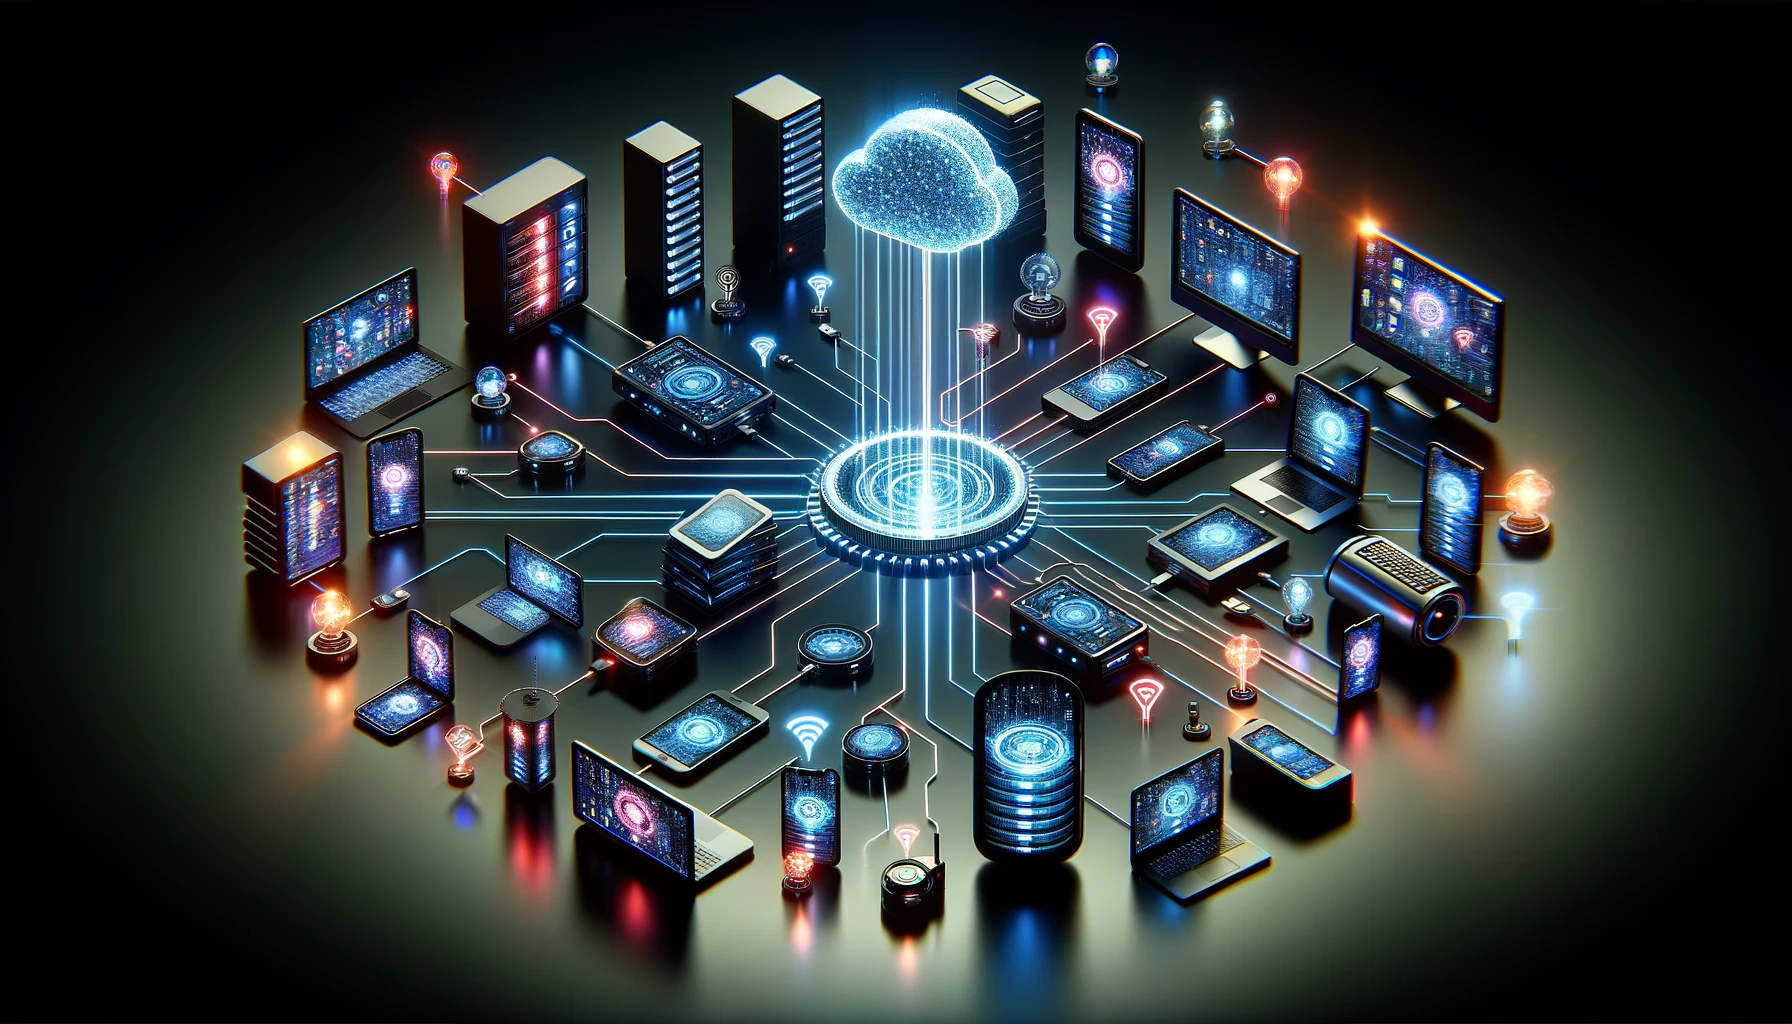
\includegraphics[width=1\textwidth]{content/1-relational-databases/figures/i1-databases-everywhere.png}
    \caption{A system of databases and services}
    \label{fig:0.i1-databases-everywhere.png}
\end{figure}

You interact every day with devices that include databases, and with services that does the same. Examples are:

\begin{itemize}
    \item Your phone and every single app on your phone
    \item Your computer and most of the applications herein.
    \item All websites you visit, such as your bank, google, etc. (few exceptions exist, but any website that is dynamic and that can save data, will most likely also use a database)
    \item Your social media
    \item Your email
    \item Your favorite online store
    \item Your favorite games
\end{itemize}

While databases are everywhere now, this was not always the case. Databases have been around for a long time, but they were not always as popular as they are now. The first databases were created in the 1960s, and were used for large scale data processing, while they slowly became more and more used, expecially at the end of 1970, and the beginning of 1980. The first relational database was created in 1970, and was called the relational model. It was created by Edgar F. Codd, and was based on the mathematical theory of sets and relations. The relational model was a huge success, and is still the most widely used database model today. The relational model was so successful, that it is often used as a synonym for relational databases, and that relational databases are often called relational models.

Initially, relational databases were predominantly utilized in substantial organizations such as banks, or for calculating salaries in major corporations. This exclusivity was due to the high cost of the computers required to operate these databases, rendering them unaffordable for the average person. However, this scenario transformed dramatically in the 1980s with the rising popularity and affordability of personal computers. As computers became more accessible, a larger segment of the population could afford to own and run a database on their personal computers. Consequently, this led to a surge in database usage, significantly increasing the demand for and creation of databases. The growth in demand meant that an ever-increasing number of people began to use databases, further amplifying their prevalence and importance in the digital world.

\section{What is SQL?}
SQL, which stands for Structured Query Language, is the cornerstone of relational databases. It's a specialized programming language designed for managing and manipulating data held in a relational database management system (RDBMS). SQL is essential for various operations within these databases, including querying, updating, and managing data.

Relational databases store data in tables, which are akin to spreadsheets with rows and columns. Each row represents a unique record, and each column a specific attribute of the data. The power of relational databases lies in their ability to efficiently organize and retrieve large volumes of data through the use of relations, typically in the form of tables.

SQL plays a pivotal role in this process. It allows users to:

\begin{itemize}
\item \textbf{Query Data:} SQL can retrieve specific data from a database through queries. For instance, if you want to find all customers from a particular city, SQL can quickly filter and display this information.
\item \textbf{Insert and Update Data:} Adding new records or updating existing ones is straightforward with SQL. It ensures data accuracy and integrity while modifying the database.
\item \textbf{Create and Modify Schema:} SQL is used to create the database structure, like tables, and modify it as needed. This includes defining the columns, data types, and constraints.
\item \textbf{Data Manipulation:} Beyond basic queries, SQL can perform complex data manipulations, combining data from multiple tables and executing sophisticated analytical functions.
\end{itemize}

One of SQL's greatest strengths is its widespread adoption and standardization. Most relational database systems use SQL, making it a crucial skill for database professionals. Its syntax and commands are relatively consistent across different database systems, with only minor variations. Understanding SQL is fundamental for anyone looking to work with relational databases, as it opens the door to efficiently managing and utilizing vast sets of data in an organized manner.

\section{What is PostgreSQL?}
PostgreSQL, often simply called Postgres, is an advanced, open-source relational database management system (RDBMS) that stands out in the vast landscape of relational databases. It's renowned for its robustness, scalability, and alignment with SQL standards. Understanding PostgreSQL in the context of relational databases involves appreciating its unique features and the reasons behind its popularity.

\begin{figure}[htbp]
    \centering
    
\includegraphics[width=0.4\textwidth]{content/1-relational-databases/figures/PostgreSQL_logo.3colors.540x557.png}
    \caption{PostgreSQL Logo}
    \label{fig:PostgreSQL_logo.3colors.540x557.png}
\end{figure}

Choosing PostgreSQL for database management comes with several advantages:

\begin{itemize}
    \item \textbf{Open Source:} Being open-source, it's free to use, modify, and distribute. This aspect makes it particularly attractive for startups and companies looking to reduce costs without sacrificing quality.
    \item \textbf{Community-Driven Development:} PostgreSQL benefits from a vibrant community that continuously contributes to its development, ensuring the database is always evolving to meet user needs.
    \item \textbf{Reliability and Stability:} It's known for its data integrity and resilience. Businesses can rely on PostgreSQL for critical applications requiring consistent uptime and robustness.
    \item \textbf{Flexibility for Developers:} PostgreSQL's support for various programming languages and its extensibility make it highly adaptable for a wide range of applications.
    \item \textbf{Scalability:} It handles large volumes of data effectively, making it suitable for businesses that anticipate growth in data volume and user load.
\end{itemize}

PostgreSQL represents a sophisticated and reliable choice within the realm of relational databases. Its adherence to SQL standards, coupled with its open-source nature, makes it a formidable tool for businesses and developers seeking a powerful, scalable, and cost-effective database solution. The most used relational database management systems are currently Oracle, MySQL (Hereunder MariaDB and other variants), Microsoft SQL Server, PostgreSQL, IBM Db2, and SQLite.

This book currently uses PostgreSQL, but will later add examples in MySQL (or variants), MSSQL and SQLite.


\section{Getting to terms with the terminology}
Understanding the realm of database systems requires familiarity with several core terminologies. Let's delve into each of these terms and explore their interrelationships.

\subsection{Overall Database Terms}
The terms one needs to understand, and how they relate to each other, are shown in \cref{fig:1.dbms-definitions.png}.


\begin{enumerate}
    \item \textbf{Database Systems:} A Database System is an integrated set of software tools that allows users to store, modify, and extract information from a database. It encompasses the DBMS software, the database itself (which includes the schema definitions and stored data), and the user application programs or queries.
    \item \textbf{User Application Programs or Queries:} User Application Programs or Queries refer to the software and commands that interact with the database system. These can range from simple query commands in SQL to complex programs written in programming languages like Python, Java, or C\#, designed to manipulate or retrieve data from the database.
    \item \textbf{DBMS Software:} DBMS Software, or Database Management System Software, is the core component of a database system. It acts as an intermediary between the user and the database. The DBMS manages the stored data, ensuring its integrity, security, and consistency. It also handles tasks such as data retrieval, update, and administration.
    \item \textbf{Schema Definitions:} Schema Definitions in a database system represent the logical structure of the entire database. They define how data is organized and how the relationships among different data elements are established. The schema includes definitions for tables, columns, data types, constraints, and relationships. It's like a blueprint for the database, dictating its organization and how the data within it is related.
    \item \textbf{Stored Data:} Stored Data is the actual data that resides in the database. This is the collection of information that has been stored in accordance with the schema definitions. Stored data can include various types of data, such as textual data, numerical data, dates, or binary data, depending on the nature of the database and its schema.
\end{enumerate}

\begin{figure}[htbp]
    \centering
    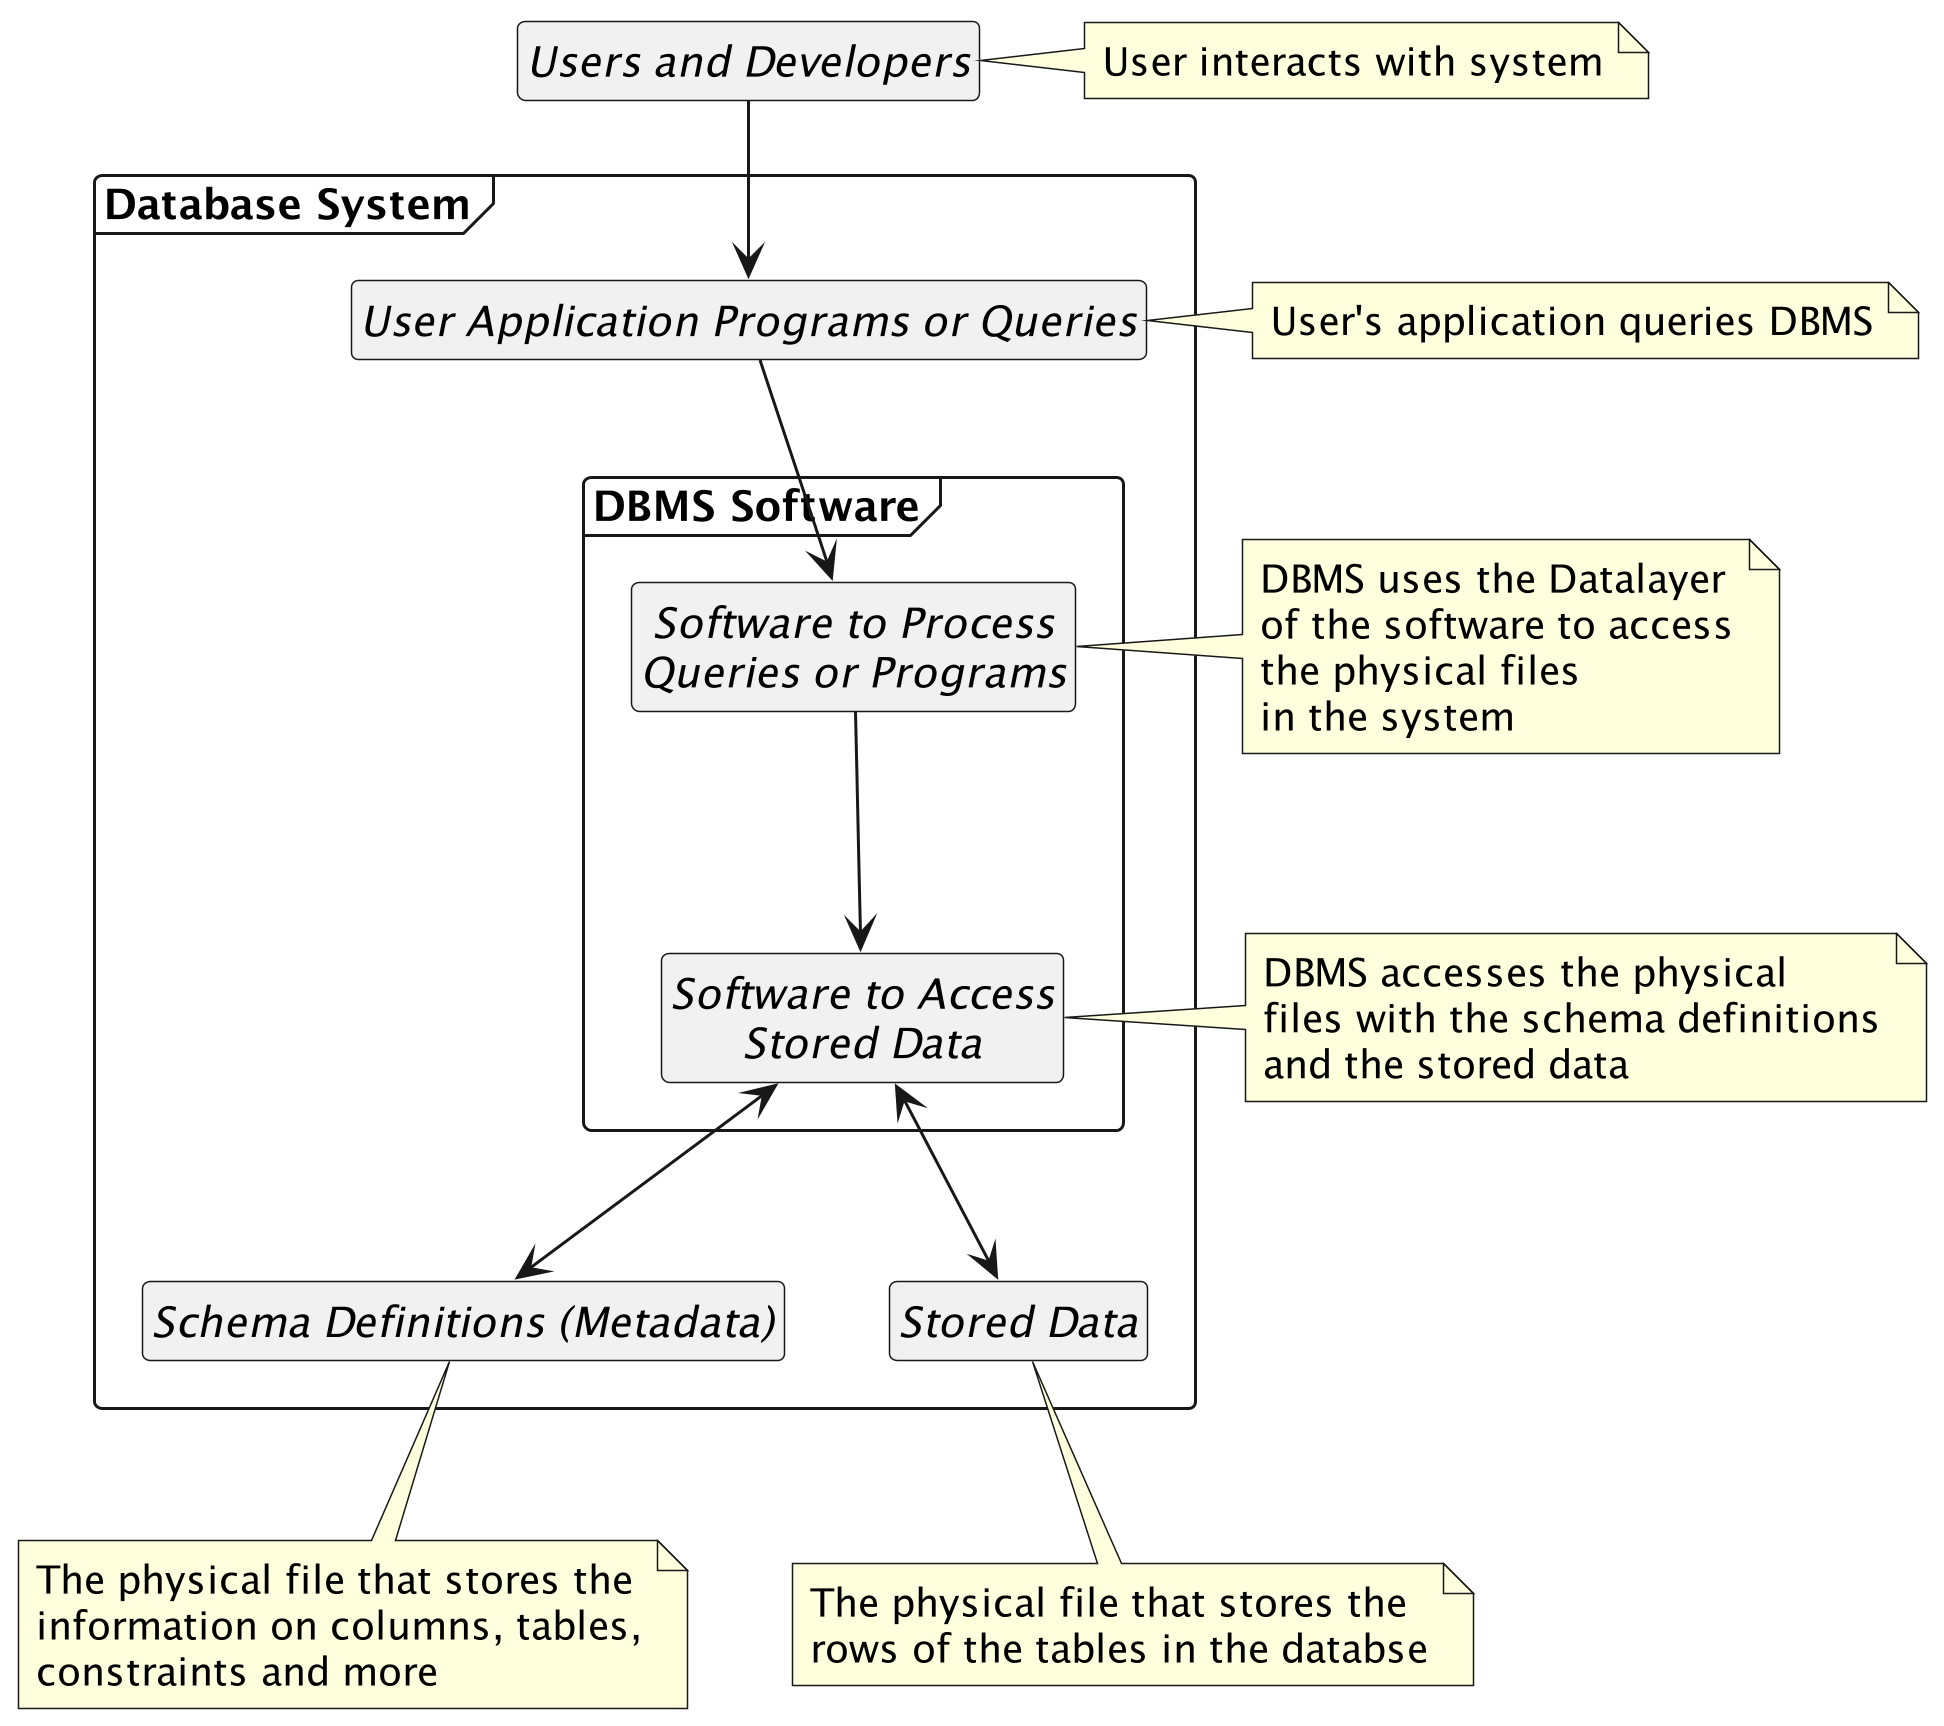
\includegraphics[width=1\textwidth]{content/1-relational-databases/figures/1.dbms-definitions.png}
    \caption{High Level Explanation of a Database Management System}
    \label{fig:1.dbms-definitions.png}
\end{figure}

The relationship among these components is hierarchical and interdependent. At the base, we have the \textbf{Stored Data}, which is the essence of the database. This data is structured and organized according to the \textbf{Schema Definitions}. The \textbf{DBMS Software} serves as the mediator between the stored data and the end-users. It uses the schema definitions to ensure data is correctly stored and retrieved. \textbf{User Application Programs or Queries} interact with the DBMS software to perform operations on the data — whether it's querying for specific information, updating records, or performing analyses. All these components together constitute the \textbf{Database System}, which is the overall environment enabling data management and utilization.


\begin{figure}[htbp]
    \centering
    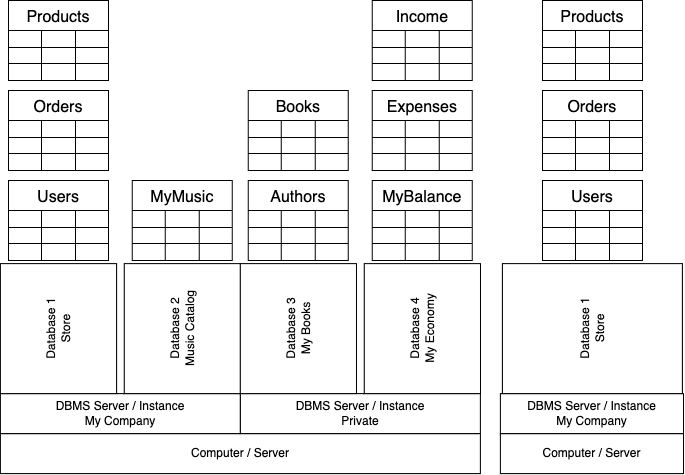
\includegraphics[width=1\textwidth]{content/1-relational-databases/figures/1.DatabaseAndTerminologyMap.drawio.png}
    \caption{Terminology extended as databases became more complex}
    \label{fig:1.dbms-content-anatomy.png}
\end{figure}

As databases became more complex, the terminology also became more complex. The terms one needs to understand, and how they relate to each other, are shown in \cref{fig:1.dbms-content-anatomy.png}. A computer, also called a server if its only purpose is to host services for other machines, can have multiple installed DBMS' of a single type. Each installation is separate, and has its own users, and listens to its own port for connections. These separatly installed DBMS' are called instances, and are typically created when a company or customer needs full rights to the DBMS system to create new users and more. Each instance of the DBMS is able to hold multiple databases. Databases can have its own users, and are normally the first tool to reach for when separating access to data, where creating new instances should only be done if separate databases does not satisfy the requirements of the system implementor. Each of theses databases, can in turn, hold multiple tables. Each table can hold multiple rows, and each row can hold multiple columns. Each column can hold multiple cells, and each cell can hold a single value.

\begin{figure}[htbp]
    \centering
    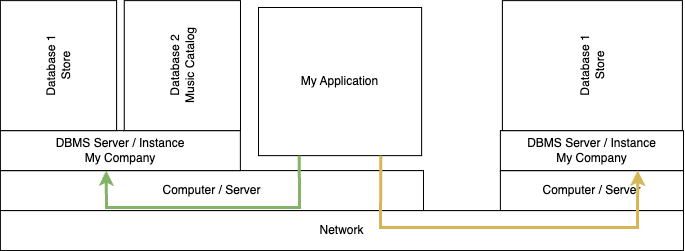
\includegraphics[width=1\textwidth]{content/1-relational-databases/figures/1.DatabasesAndConnecting.drawio.png}
    \caption{How do we connect to the database?}
    \label{fig:1.dbms-connection-explained.png}
\end{figure}

To connect to the database we want, an application would need to either connect to an instance on the localhost, or an instance on another server. in \cref{fig:1.dbms-connection-explained.png}, we explore how this works. The green arrow would be connecting to a DBMS server within the same physical machine, also often called localhost. It tends to be called localhost, as localhost will always resolve to 127.0.0.1, which is the loopback, that is always the computer you are on. The application will need to create a connection string, and this string contains the IP (in this case localhost), the user, the password, and the name of the database the application wishes to connect to. When following the yellow arrow though, we are trying to connect to a different computer to get our data. For this, we need the same information as before, but the application now needs the IP from the remote server in the connection string. Once that detail is changed, the connection can now commence, but the connection will be slower, as the data needs to traverse the network. An application will need multiple connection strings and connections over the network if it wants data from multiple databases, or from multiple instances.

\subsection{The anatomy of a table}
As can be seen in \cref{fig:2.table-definitions.png}, a table is structured through a series of rows and columns that intersect to form cells. Each column in the table is headed by an attribute, which is also commonly referred to as a field, column, or property. These attributes represent the data categories within the table, defining the kind of data each column holds. Similarly, each row in the table is known as a tuple, which can alternatively be called a row, record or an entry. Tuples are instances of the data, encompassing a unique set of values for the attributes defined by the columns. Together, attributes and tuples constitute the fundamental framework of a table.

\begin{figure}[htbp]
    \centering
    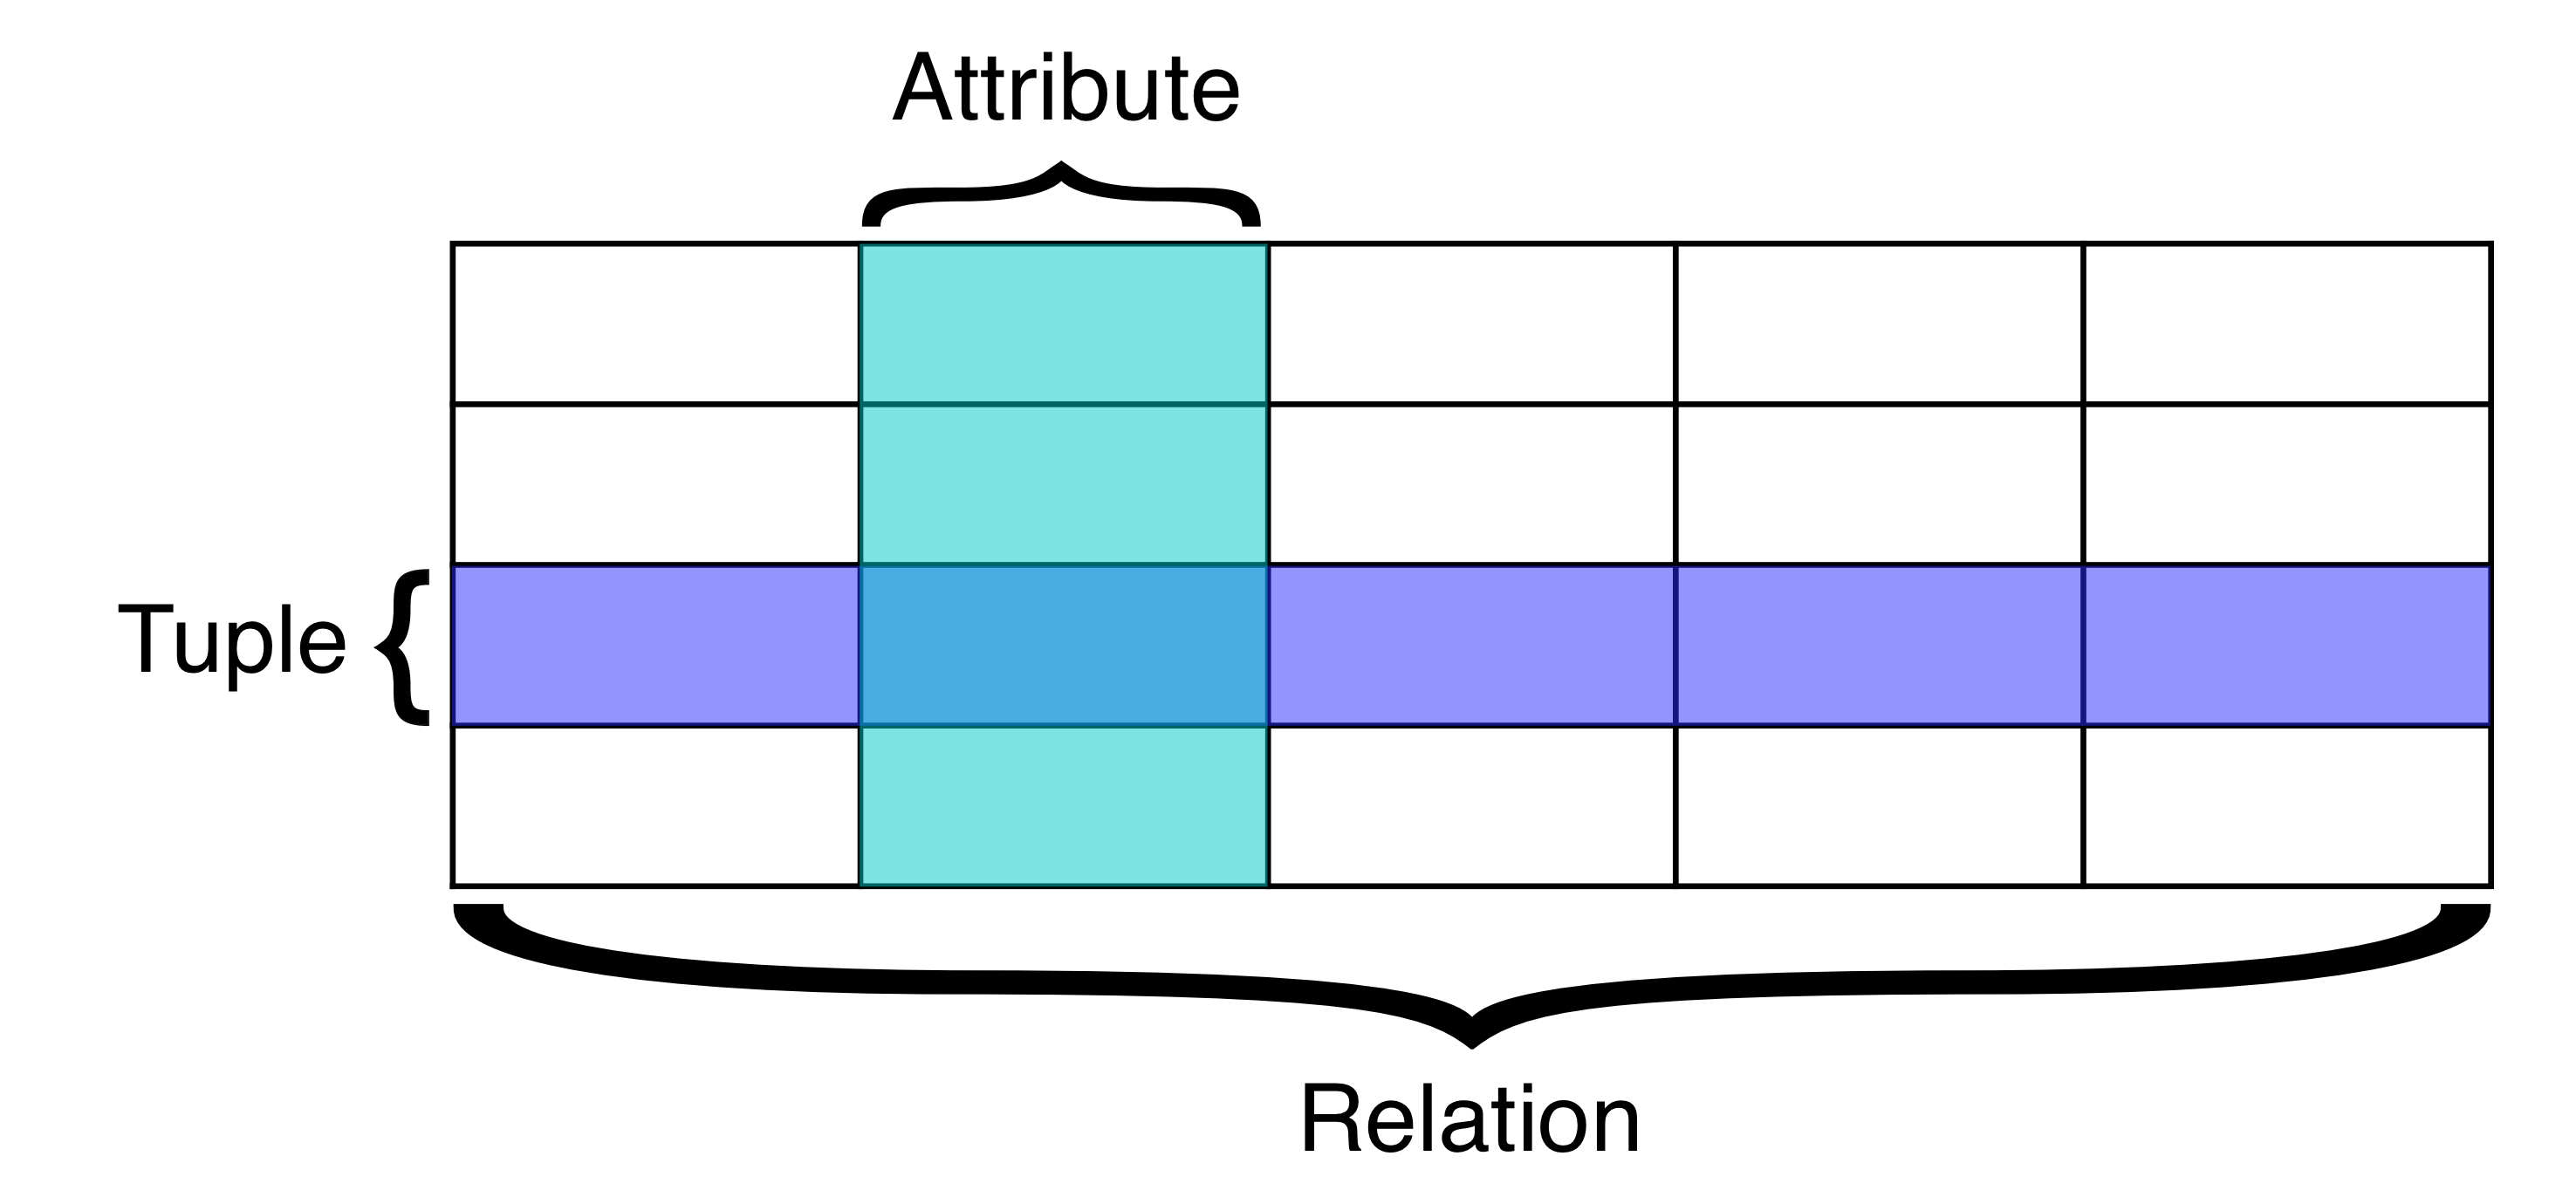
\includegraphics[width=1\textwidth]{content/1-relational-databases/figures/2.table-definitions.png}
    \caption{Table Terminology (Artist: Chris Martin)}
    \label{fig:2.table-definitions.png}
\end{figure}

\section{Setting up your machine}
Before you can start working with databases, you need to set up your machine. This section will guide you through the process of setting up your machine, and installing the required software.

\subsection{Windows Specific Instructions}
Go to \url{https://www.enterprisedb.com/downloads/postgres-postgresql-downloads} and download the latest version of PostgreSQL. 
\begin{figure}[htb]
    \centering
    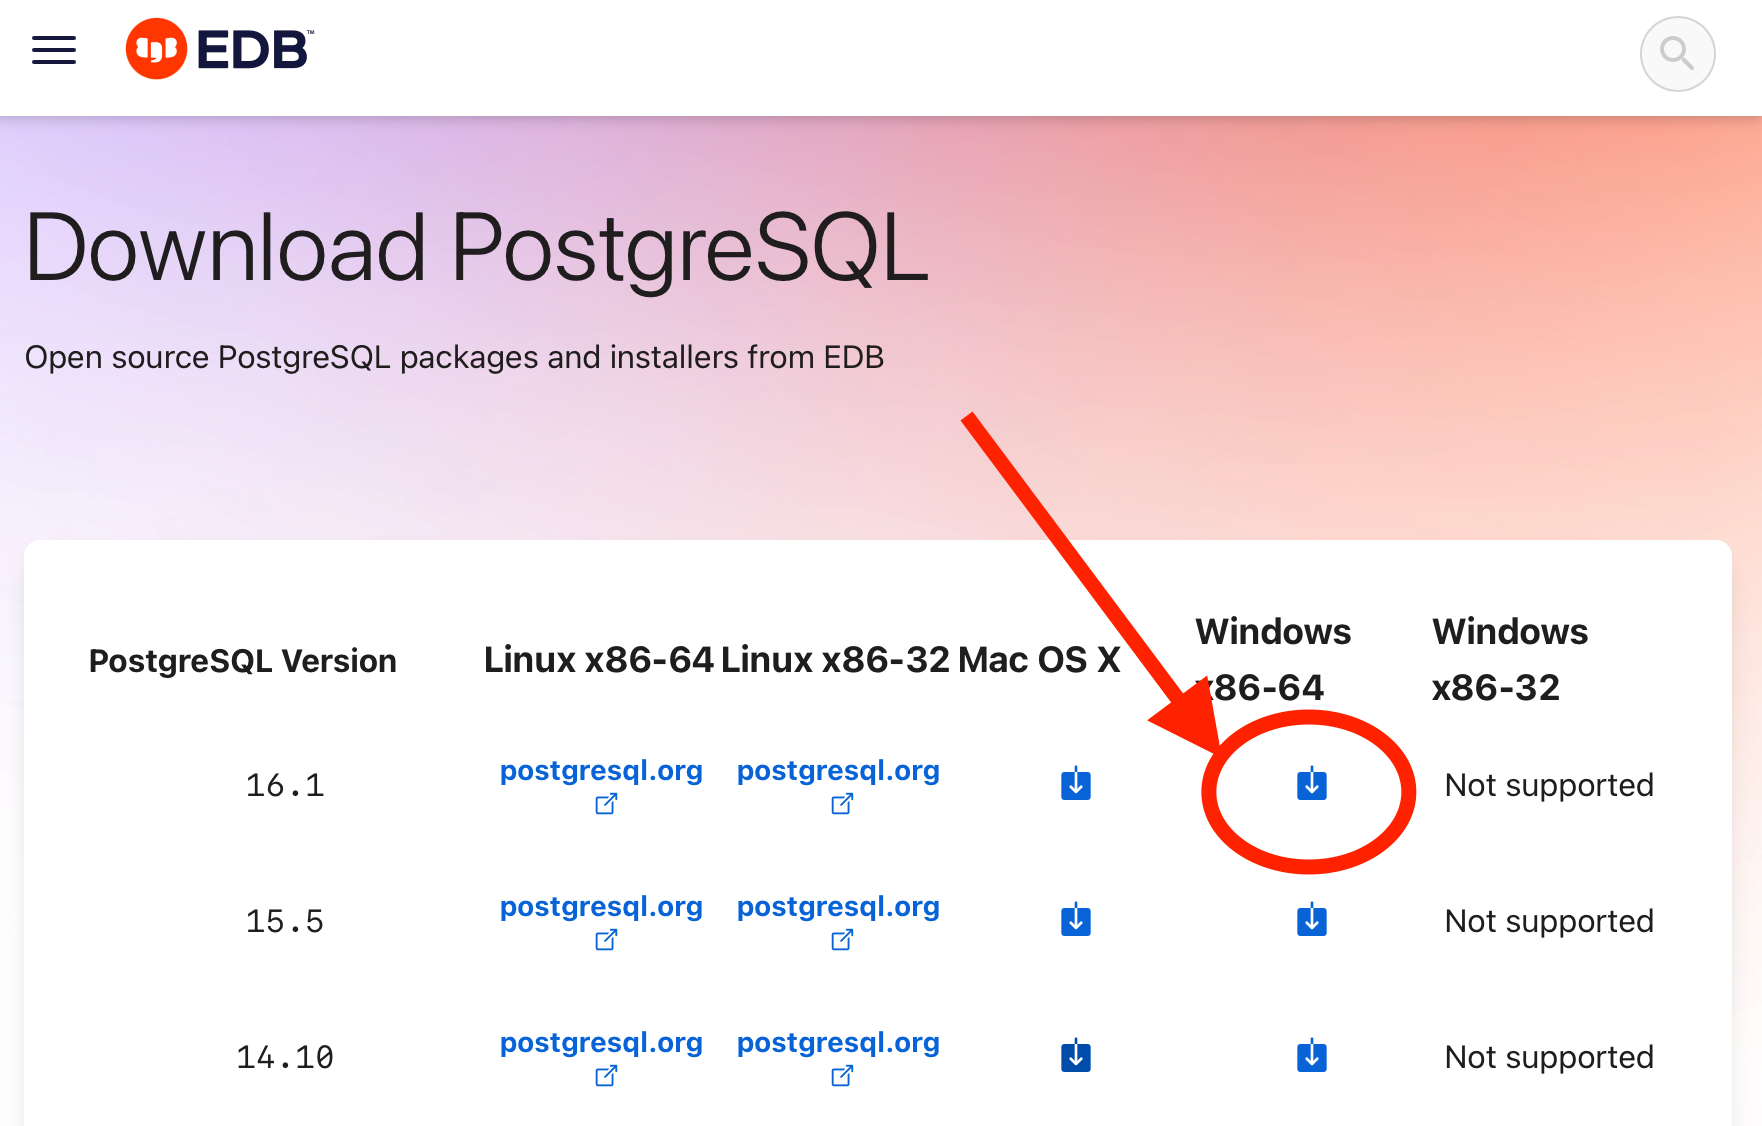
\includegraphics[width=1\textwidth]{content/1-relational-databases/figures/1.install-for-windows-1.png}
    \caption{Download location for PostgreSQL}
    \label{fig:1.postgresql-download-1.png}
\end{figure}

Run the installer, and follow the instructions, but be sure to deselect "Stack Builder" (see \cref{fig:1.postgresql-download-2.png}), as we will not be using it in this book. 

\begin{figure}[htb]
    \centering
    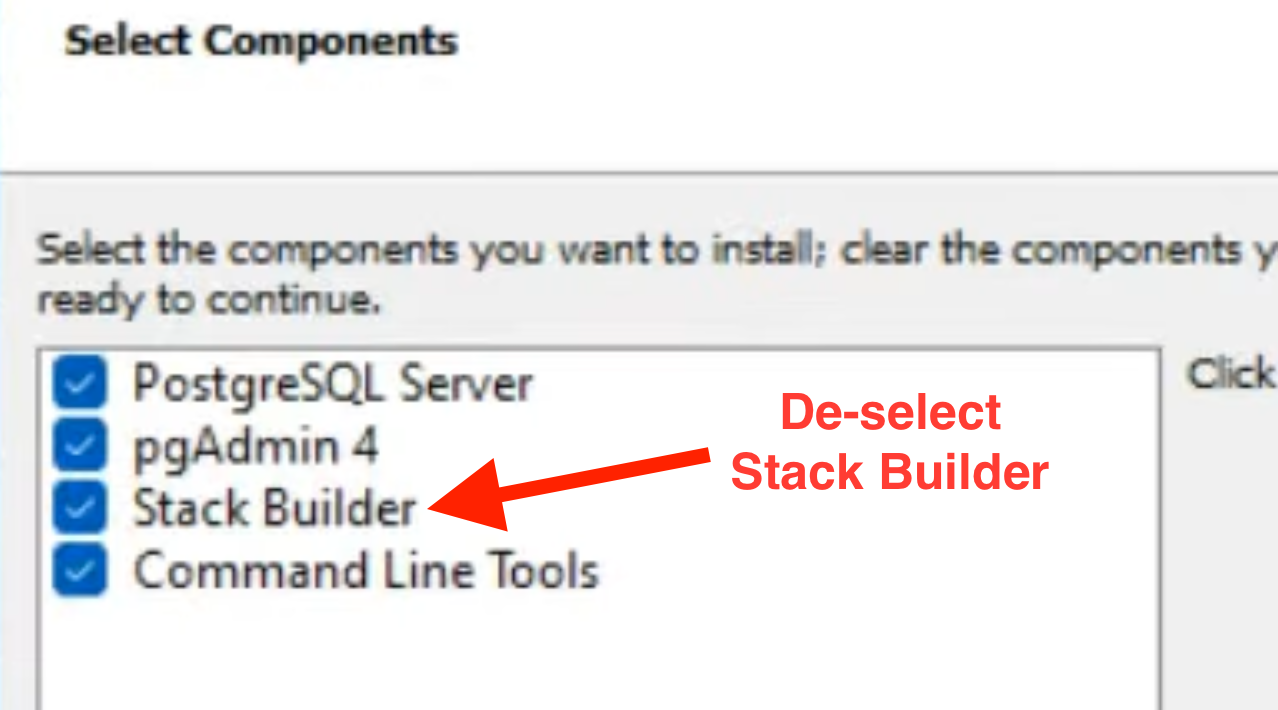
\includegraphics[width=0.6\textwidth]{content/1-relational-databases/figures/1.install-for-windows-2.png}
    \caption{Components to install}
    \label{fig:1.postgresql-download-2.png}
\end{figure}

When asked for a password, use the password you want to use for the postgres user. This is the user that is used to manage the database server. Be sure to remember this password, as you will need it later. After this password it set, the database server instance will have the user postgres, and the password will be what you set. Beware that your computers password, the database server instance password, and the pgAdmin password are all different passwords.

\begin{figure}[htb]
    \centering
    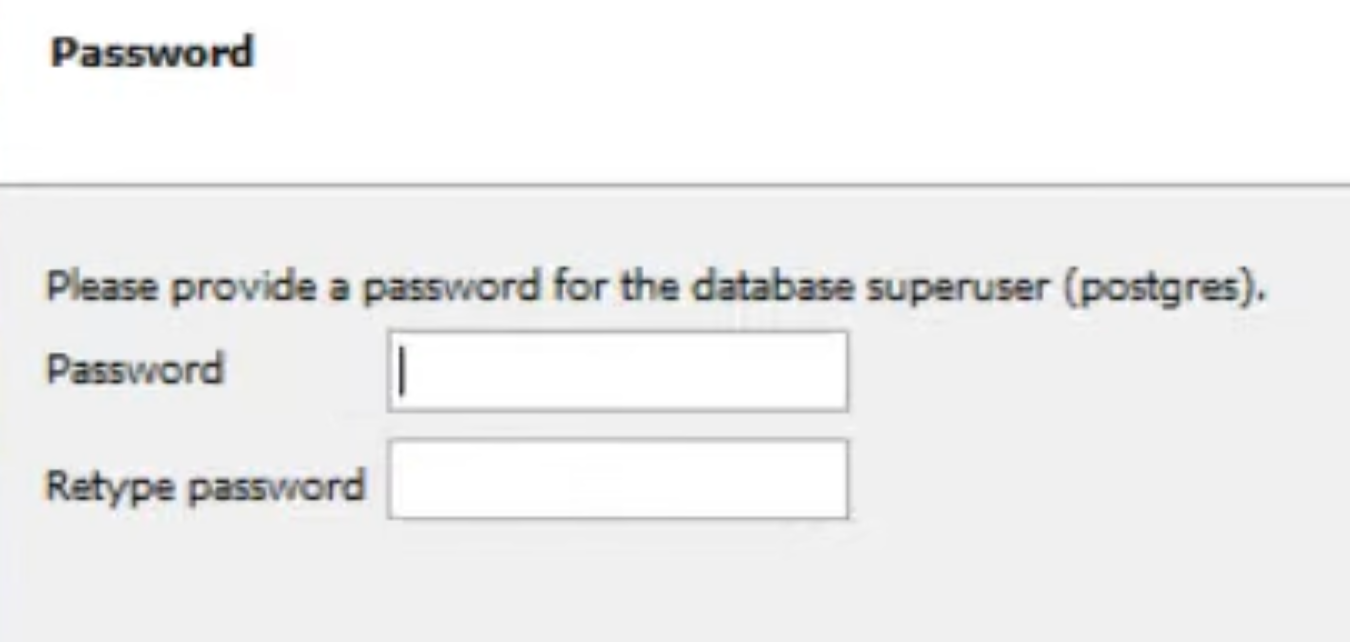
\includegraphics[width=0.7\textwidth]{content/1-relational-databases/figures/1.install-for-windows-3.png}
    \caption{Pick a password for the postgres user}
    \label{fig:1.postgresql-download-3.png}
\end{figure}


This is not the password you will use to connect to the database server, but the password you will use to manage the database server. This password is not used in this book, but it is good practice to set it to something you can remember.

\subsection{Mac Specific Instructions}
Installation of PostgreSQL on a Mac is done through the terminal. You can pick any way to do this, but we are going to use the homebrew (https://brew.sh) solution. Open the terminal, and run the following command to install homebrew: 

\begin{minted}[fontsize=\footnotesize]{bash}
    /bin/bash -c "$(curl -fsSL https://raw.githubusercontent.com
        /Homebrew/install/HEAD/install.sh)"
\end{minted}

Or copy it directly from the frontpage of the homebrew website. After homebrew is installed, you can install PostgreSQL by running the following command in the terminal:

\begin{minted}[fontsize=\footnotesize]{bash}
    brew install postgresql
    /opt/homebrew/bin/createuser -s postgres
\end{minted}

After PostgreSQL is installed, you can start the server by running the following command in the terminal:

\begin{minted}[fontsize=\footnotesize]{bash}
    brew services start postgresql
\end{minted}

This will start the PostgreSQL server, and it will start automatically every time you start your computer. If you want to stop the server, you can run the following command in the terminal:

\begin{minted}[fontsize=\footnotesize]{bash}
    brew services stop postgresql
\end{minted}

And if you only want to start the server once, you can run the following command in the terminal:

\begin{minted}[fontsize=\footnotesize]{bash}
    brew services run postgresql
\end{minted}


PostgreSQL will not have a password set at this point, and a password needs to be set using the comandline. It can be set by running the following command in the terminal:

\begin{minted}[fontsize=\footnotesize]{bash}
    psql postgres
    \password postgres
\end{minted}

Running the above code will prompt you to write a password for the postgres user. Remember this password, as you will need it every time you connect to the database server instance. 


Remember to also install pgAdmin using homebrew, by running the following command in the terminal:
\begin{minted}[fontsize=\footnotesize]{bash}
    brew install pgadmin4
\end{minted}

At the first run of pgadmin a password needs to be set. Remember it, as you need it every time you used pgadmin. Be aware that this password is not the same as the password for the database server instance, and the password for the postgres user.


\subsection{Linux Specific Instructions}
With linux, you are mostly on your own, but generally, most linux distributions have a package manager that you can use to install PostgreSQL. The package manager is different from distribution to distribution, but the most common ones are apt, yum, and dnf. To install PostgreSQL on Ubuntu, you can run the following command in the terminal:

\begin{minted}[fontsize=\footnotesize]{bash}
    sudo apt-get install postgresql
\end{minted}

After PostgreSQL is installed, you can start the server by running the following command in the terminal:

\begin{minted}[fontsize=\footnotesize]{bash}
    sudo systemctl start postgresql
\end{minted}

This will start the PostgreSQL server, and it will start automatically every time you start your computer. If you want to stop the server, you can run the following command in the terminal:

\begin{minted}[fontsize=\footnotesize]{bash}
    sudo systemctl stop postgresql
\end{minted}

PostgreSQL will not have a password set at this point, and a password needs to be set using the comandline. It can be set by running the following command in the terminal:

\begin{minted}[fontsize=\footnotesize]{bash}
    psql postgres
    \password postgres
\end{minted}

Running the above code will prompt you to write a password for the postgres user. Remember this password, as you will need it every time you connect to the database server instance. 
Remember to install pgAdmin too. This can be done using the package manager of your distribution. With Ubuntu, you can run the following command in the terminal:

\begin{minted}[fontsize=\footnotesize]{bash}
    sudo apt-get install pgadmin4
\end{minted}

At the first run of pgadmin a password needs to be set. Remember it, as you need it every time you used pgadmin. Be aware that this password is not the same as the password for the database server instance, and the password for the postgres user.

\section{Connecting to the database with pgAdmin}
When you have installed PostgreSQL, you can connect to the database using pgAdmin. pgAdmin is a graphical user interface that allows you to interact with the database. It is a powerful tool that allows you to create, manage, and query databases. This section will guide you through the process of connecting to the database using pgAdmin.

First start the application in your respective operating system. The application will look like \cref{fig:1.pgadmin1}.
\begin{figure}[H]
    \centering
    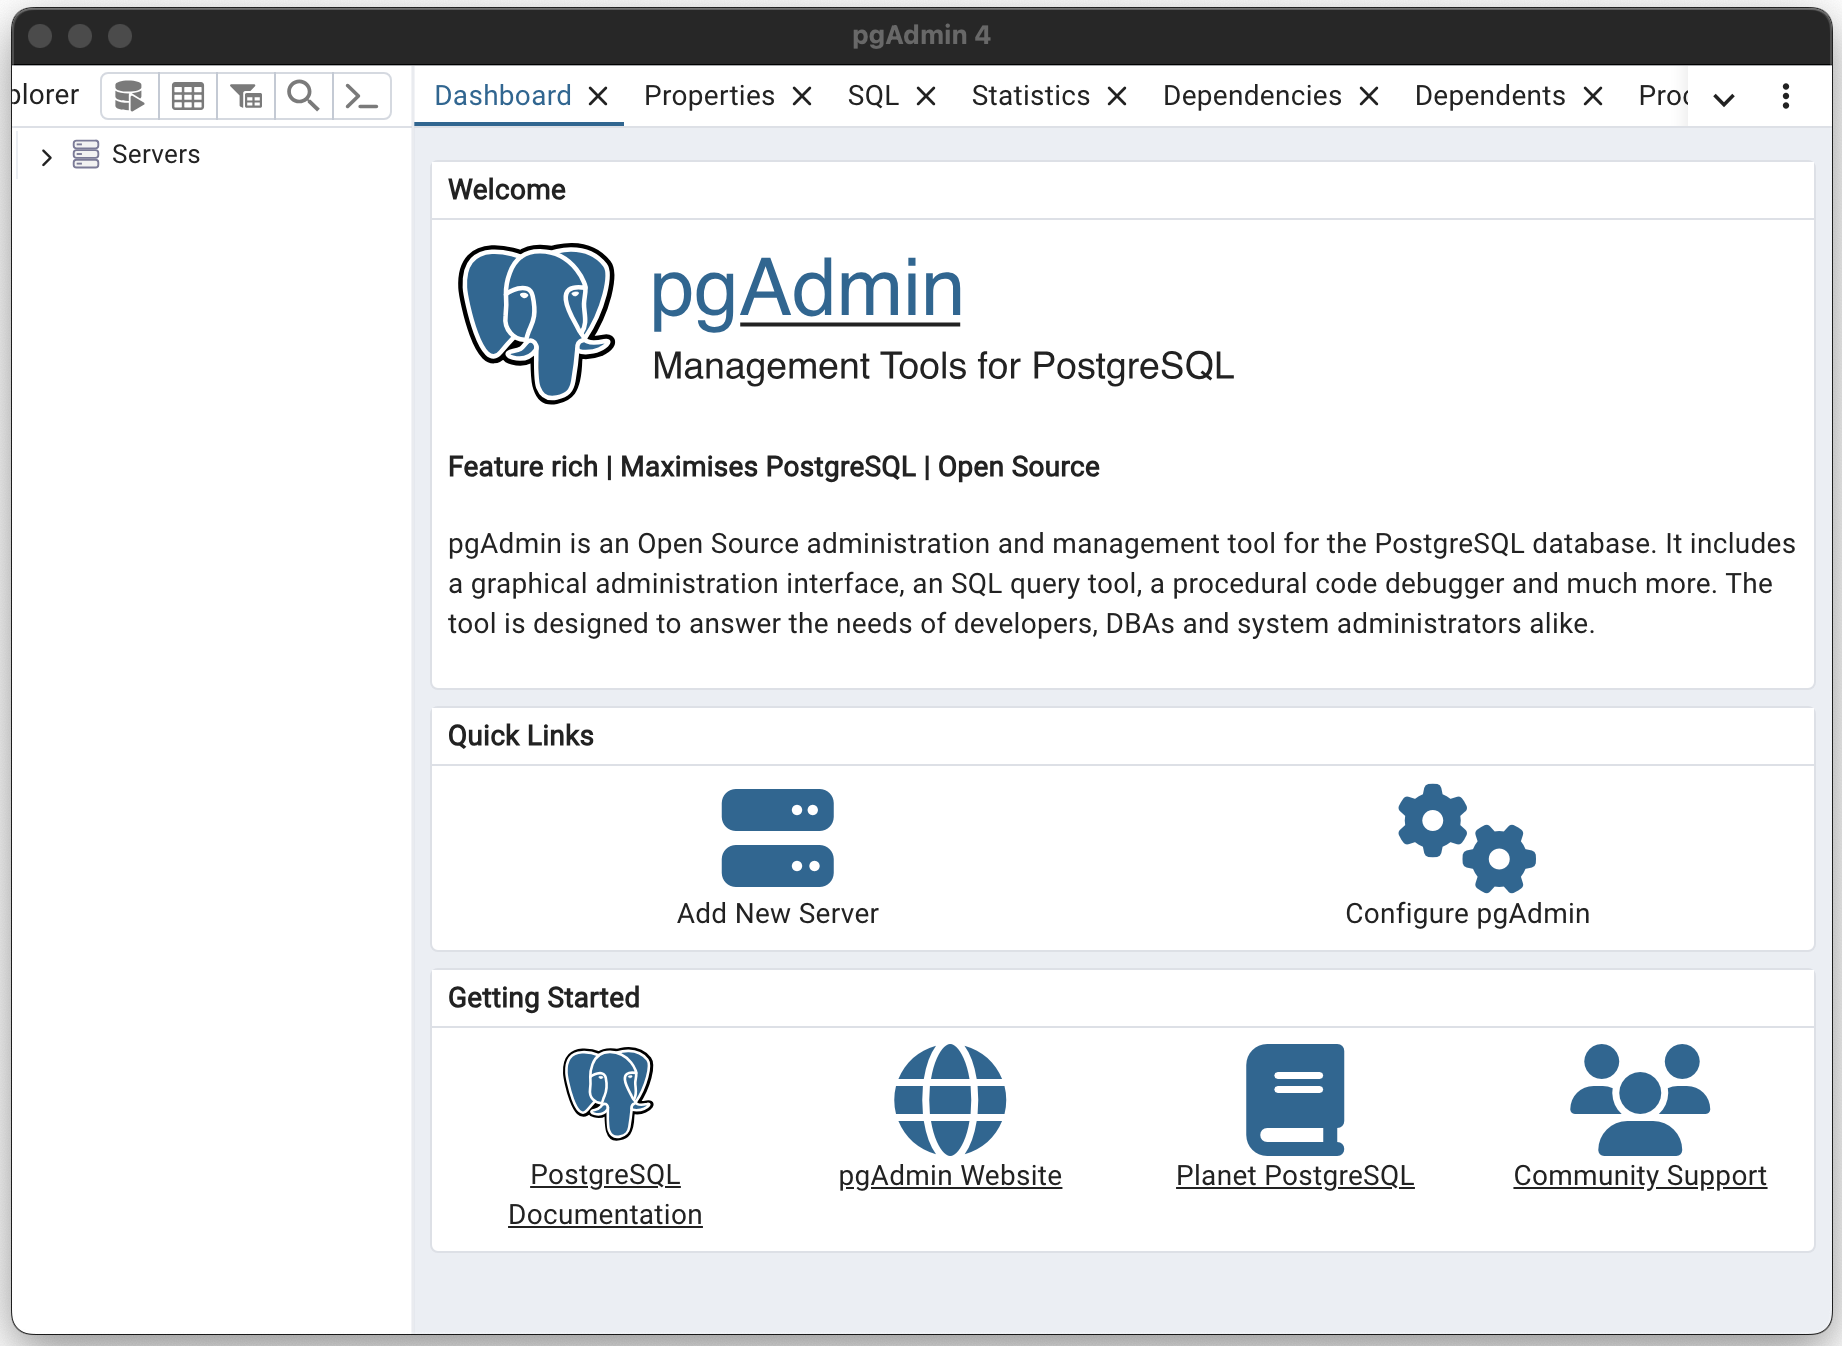
\includegraphics[width=0.7\textwidth]{content/1-relational-databases/figures/pgadmin/1.png}
    \caption{Starting pgAdmin}
    \label{fig:1.pgadmin1}
\end{figure}

Next, you need to register a server. This is done by right clicking on the "Servers" node in the tree view, and selecting "Create" and then "Server...". This will open a dialog where you can fill in the connection information. The dialog will look like \cref{fig:1.pgadmin2}.

\begin{figure}[H]
    \centering
    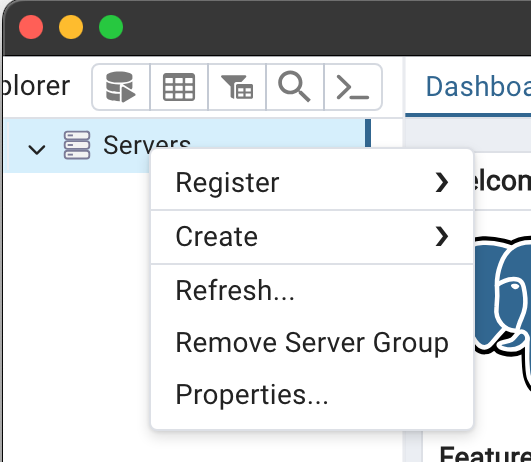
\includegraphics[width=0.3\textwidth]{content/1-relational-databases/figures/pgadmin/2.png}
    \caption{Initiate registration of a server}
    \label{fig:1.pgadmin2}
\end{figure}


% The dialog will look like \cref{fig:1.pgadmin3}.

% \begin{figure}[H]
%     \centering
%     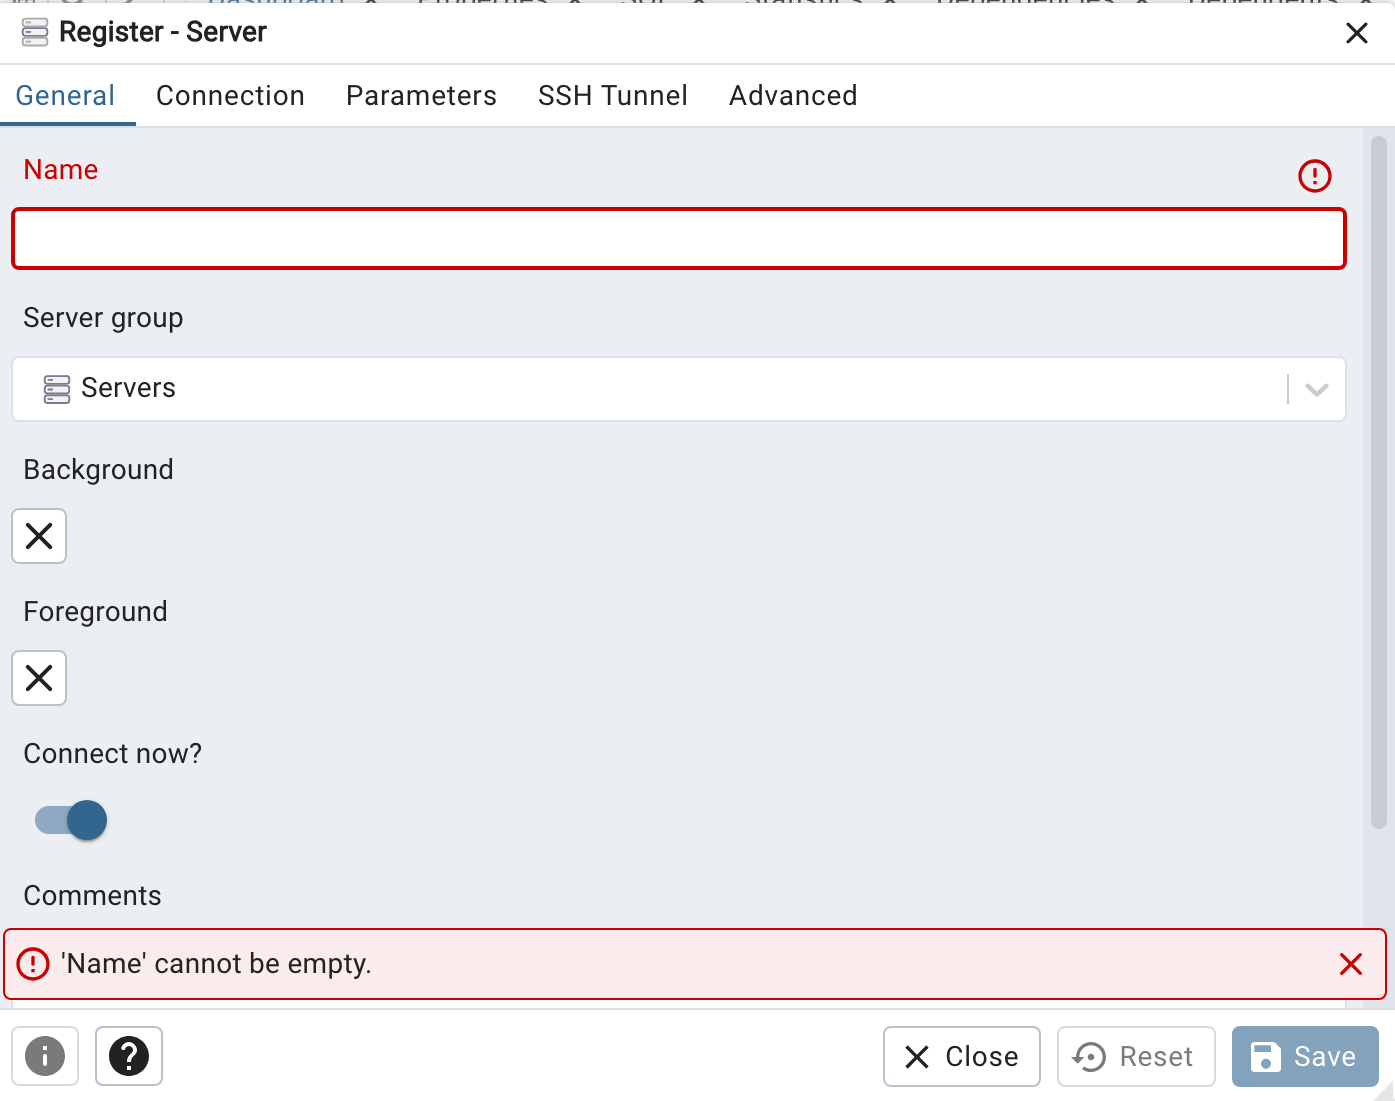
\includegraphics[width=0.6\textwidth]{content/1-relational-databases/figures/pgadmin/3.png}
%     \caption{Pick a name, i recommend localhost}
%     \label{fig:1.pgadmin3}
% \end{figure}

Pick a name for the server, and click save. I recommend localhost, as it is the default name, and as it refers to your local computer. This is convention for development machines. 
Move to the tab "Connection", and fill in the connection information. The hostname is localhost, the username is postgres, and the password is the password you set for the postgres user. The dialog will look like \cref{fig:1.pgadmin4}.

\begin{figure}[H]
    \centering
    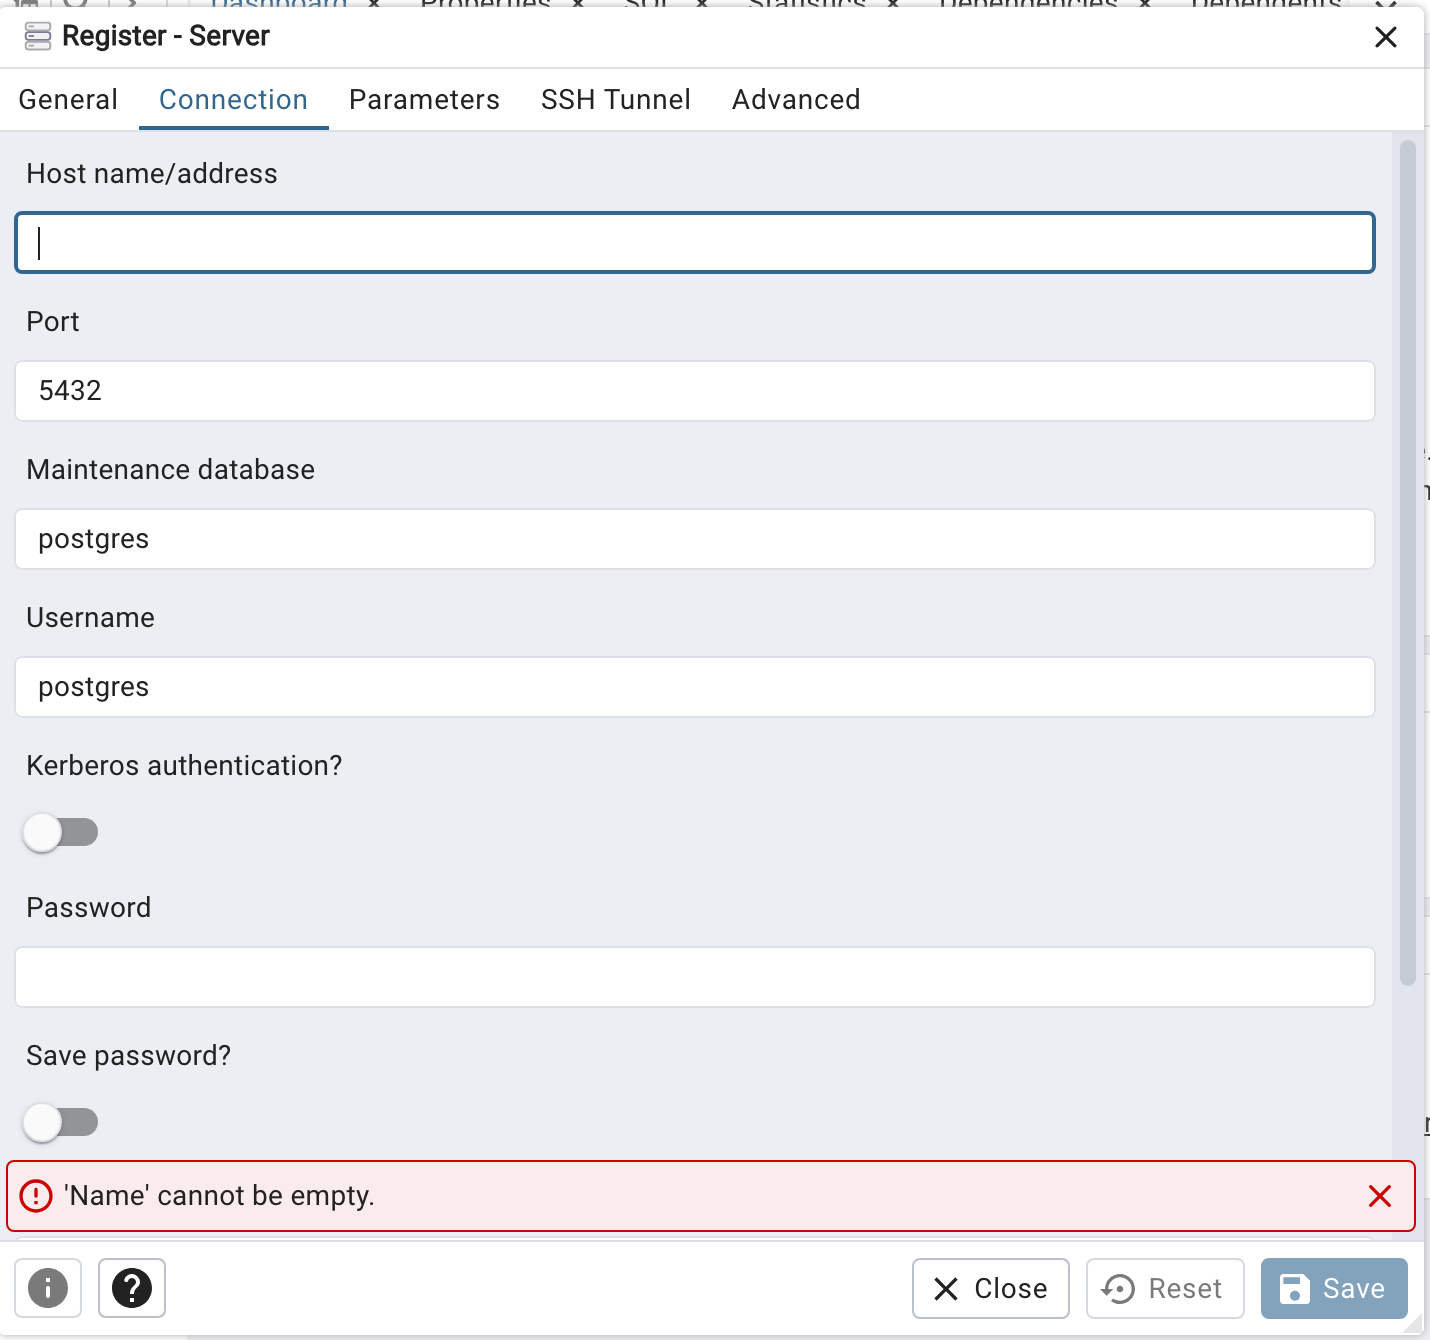
\includegraphics[width=0.6\textwidth]{content/1-relational-databases/figures/pgadmin/4.png}
    \caption{Fill in connection information, hostname is localhost, username is postgres, and the password is the password you set for the postgres user}
    \label{fig:1.pgadmin4}
\end{figure}

% If you have filled in the information correctly, you will see a success message like \cref{fig:1.pgadmin5}. If you see this message, you have successfully connected to the database server instance.

% \begin{figure}[h]
%     \centering
%     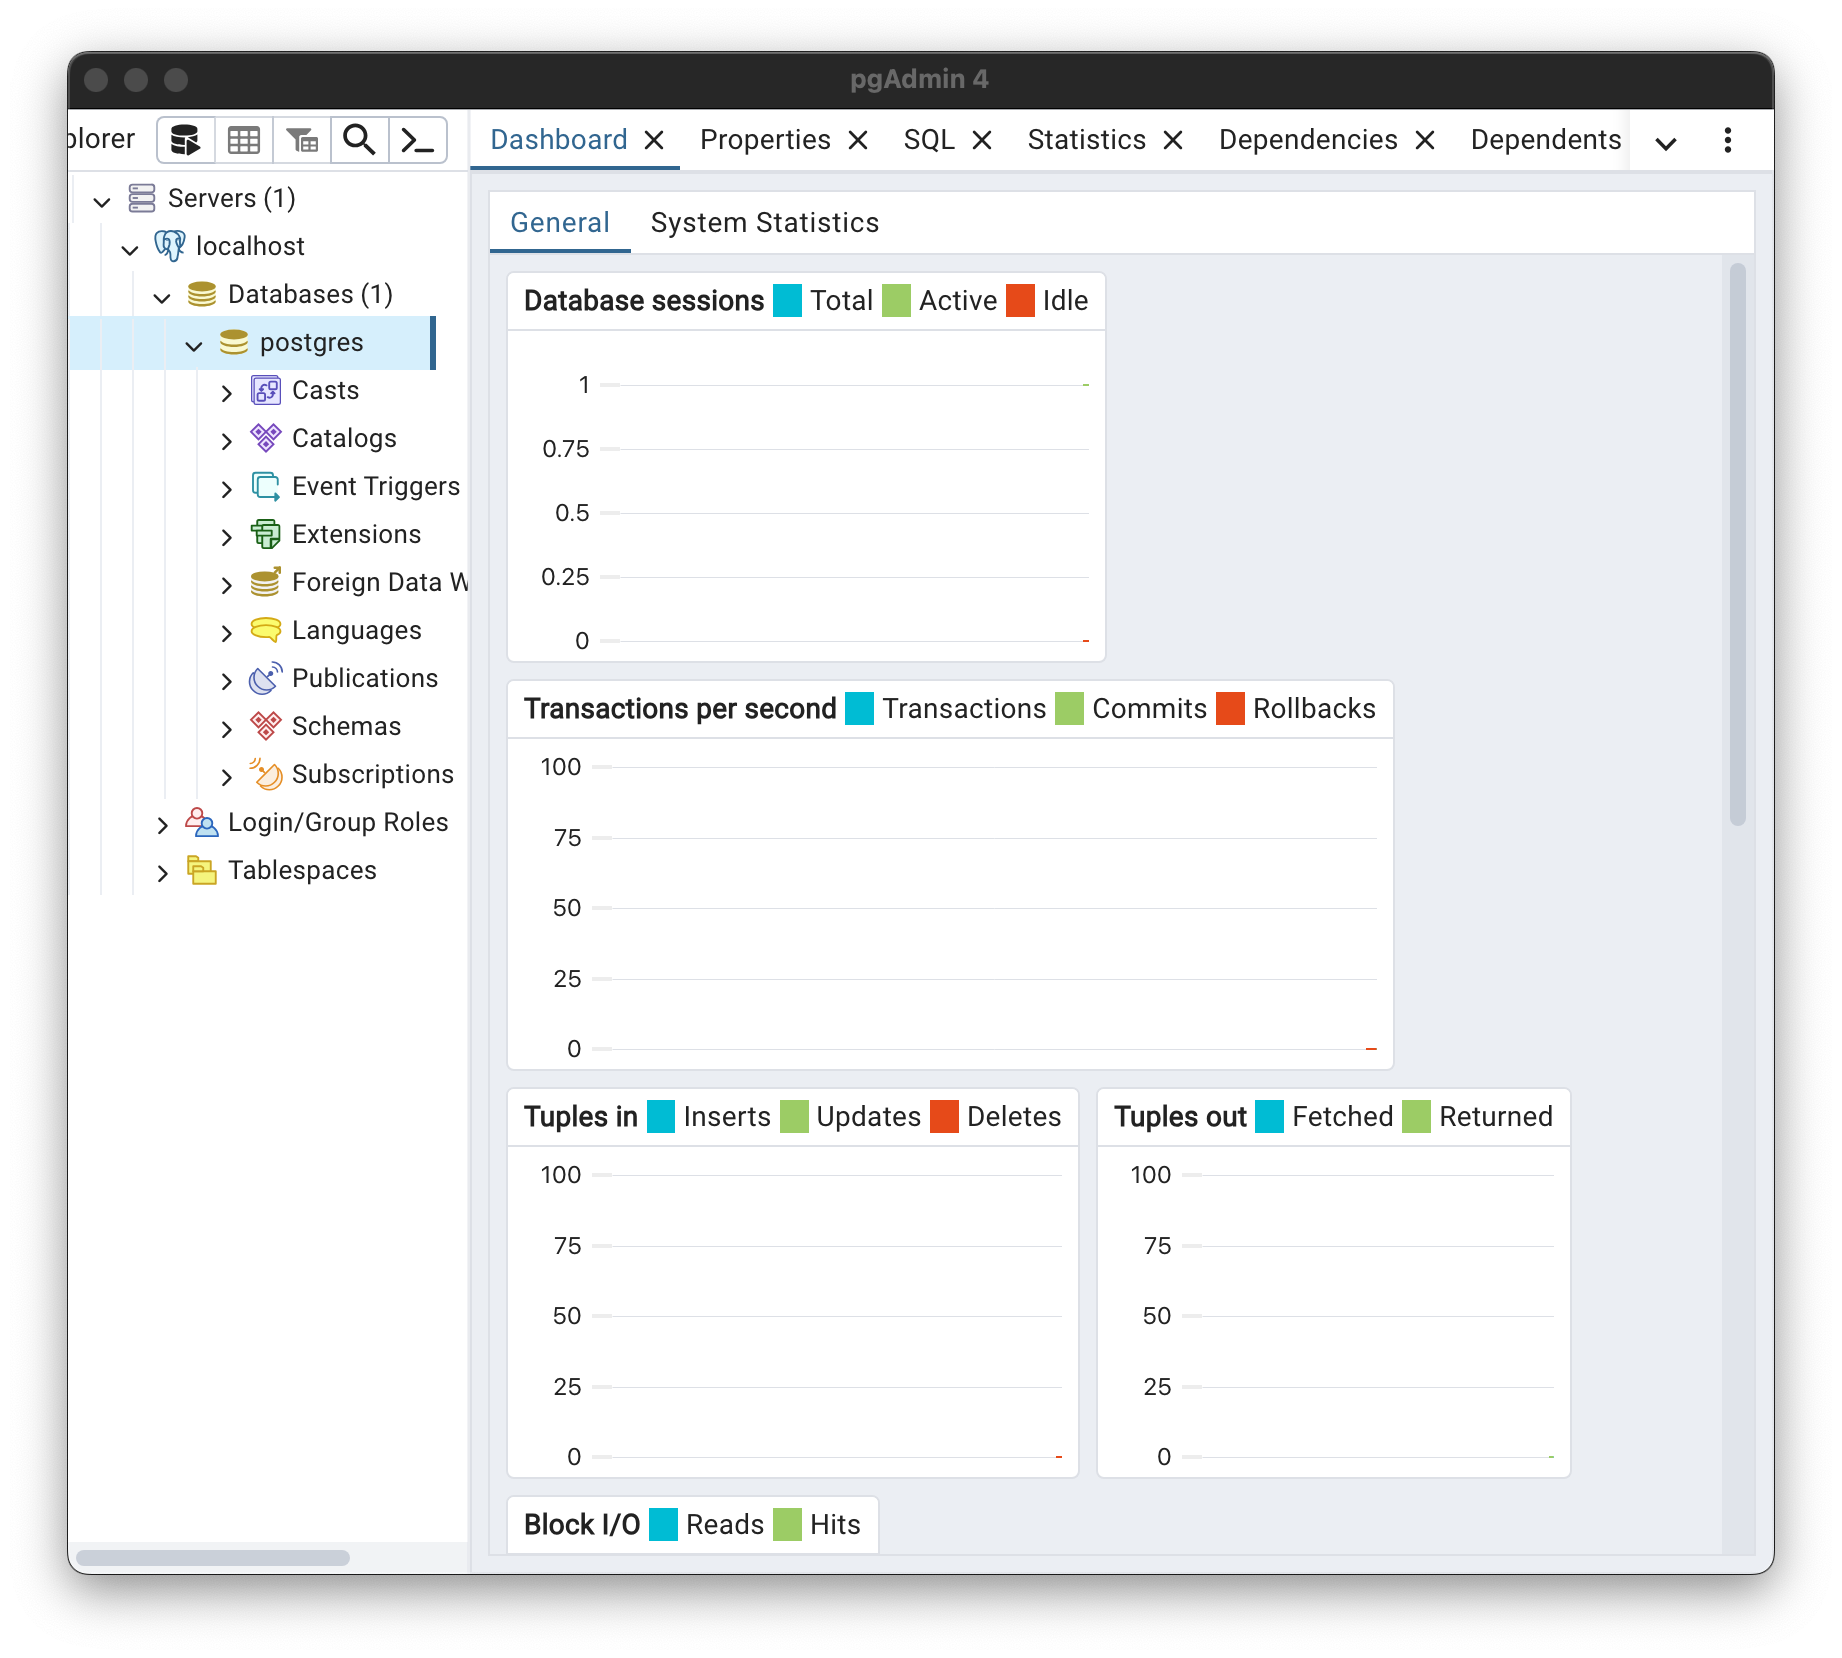
\includegraphics[width=0.7\textwidth]{content/1-relational-databases/figures/pgadmin/5.png}
%     \caption{Success looks like this!}
%     \label{fig:1.pgadmin5}
% \end{figure}
You should now be connected to the database and see it in the right pane.
Now you can create a new database. This is done by right clicking on the "Databases" node in the tree view, and selecting "Create" and then "Database...". This will open a dialog where you can fill in the database information. The dialog will look like \cref{fig:1.pgadmin6}.

\begin{figure}[H]
    \centering
    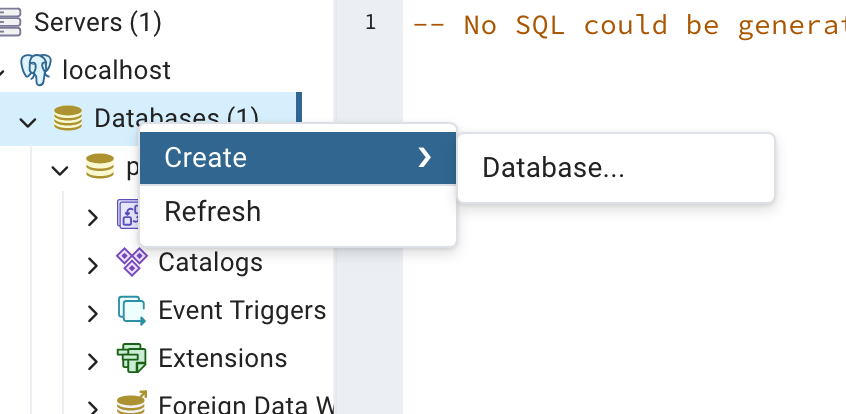
\includegraphics[width=0.5\textwidth]{content/1-relational-databases/figures/pgadmin/6.png}
    \caption{Creating a new database from pgAdmin}
    \label{fig:1.pgadmin6}
\end{figure}

Pick a name for the database, and click save. The dialog will look like \cref{fig:1.pgadmin7}.

\begin{figure}[H]
    \centering
    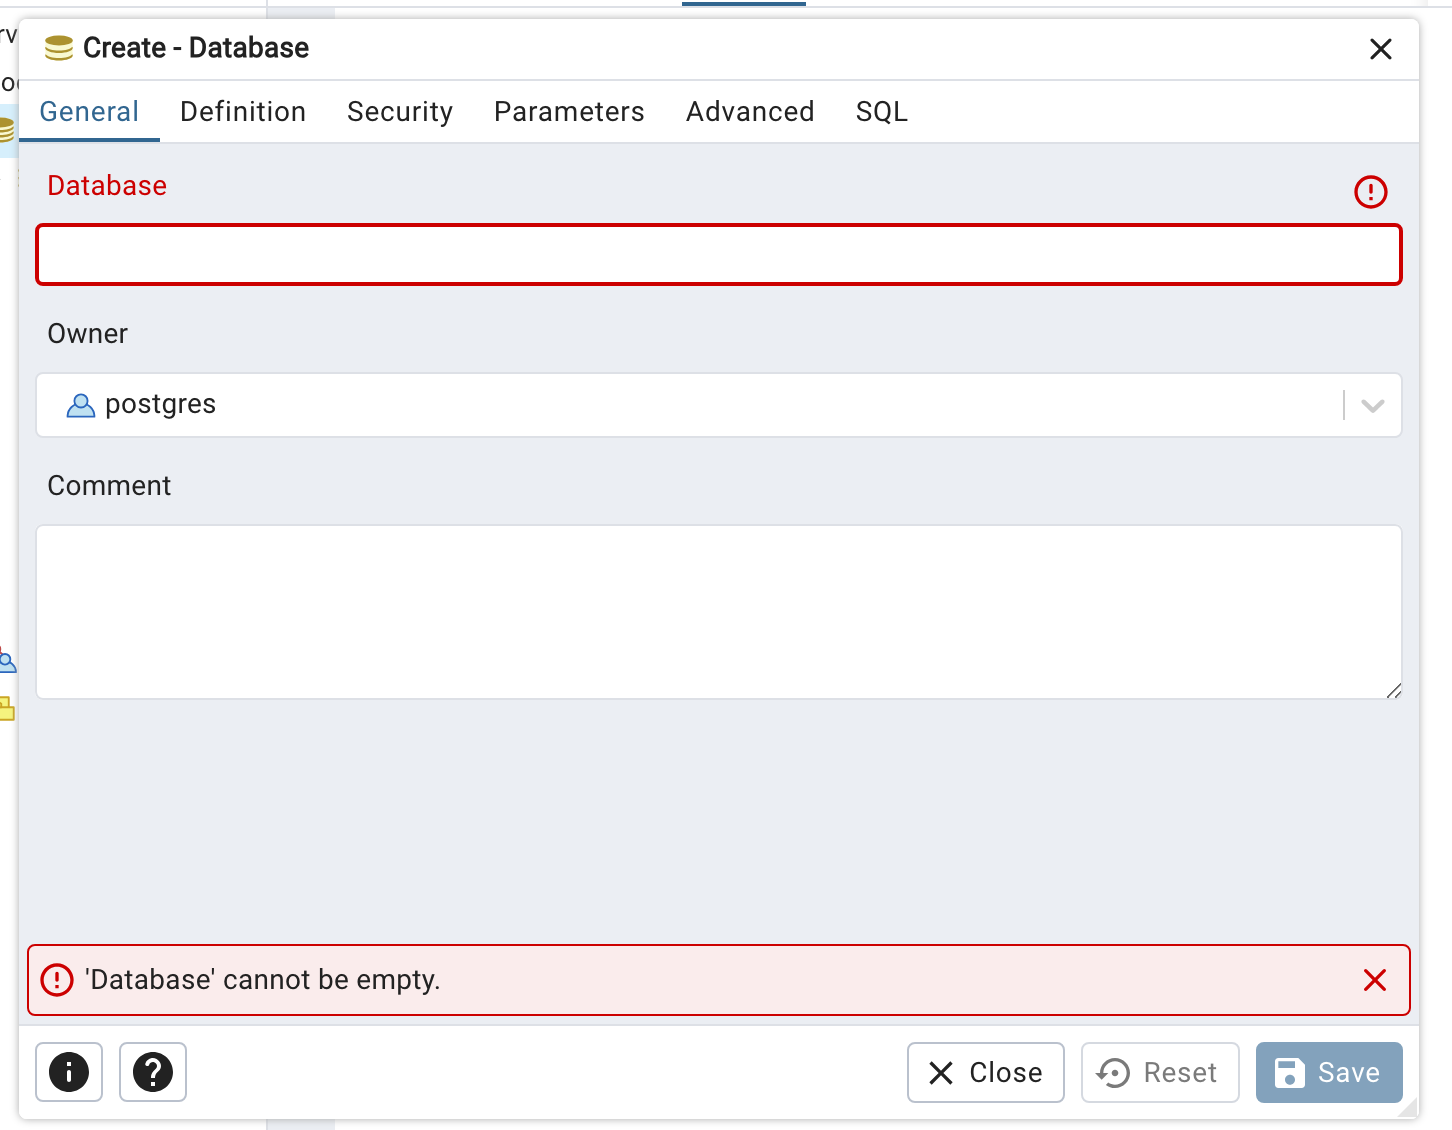
\includegraphics[width=0.7\textwidth]{content/1-relational-databases/figures/pgadmin/7.png}
    \caption{Pick a database name, and click save}
    \label{fig:1.pgadmin7}
\end{figure}

Now you have created a database, and you can start working with it. You can start by creating tables, and inserting data into the tables. This is done by right clicking on the database, and selecting "Query Tool". This will open a dialog where you can write your code, and execute it. The dialog will look like \cref{fig:1.pgadmin8}.

\begin{figure}[H]
    \centering
    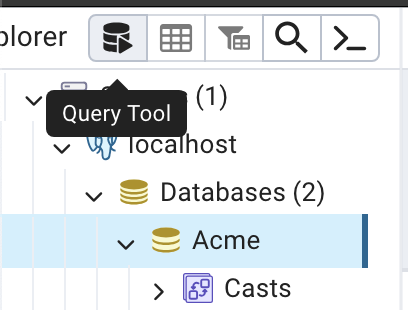
\includegraphics[width=0.4\textwidth]{content/1-relational-databases/figures/pgadmin/8.png}
    \caption{Mark the database, and press the query tool}
    \label{fig:1.pgadmin8}
\end{figure}

Write your code, and execute it. The dialog will look like \cref{fig:1.pgadmin9}. You are now ready for coding.

\begin{figure}[H]
    \centering
    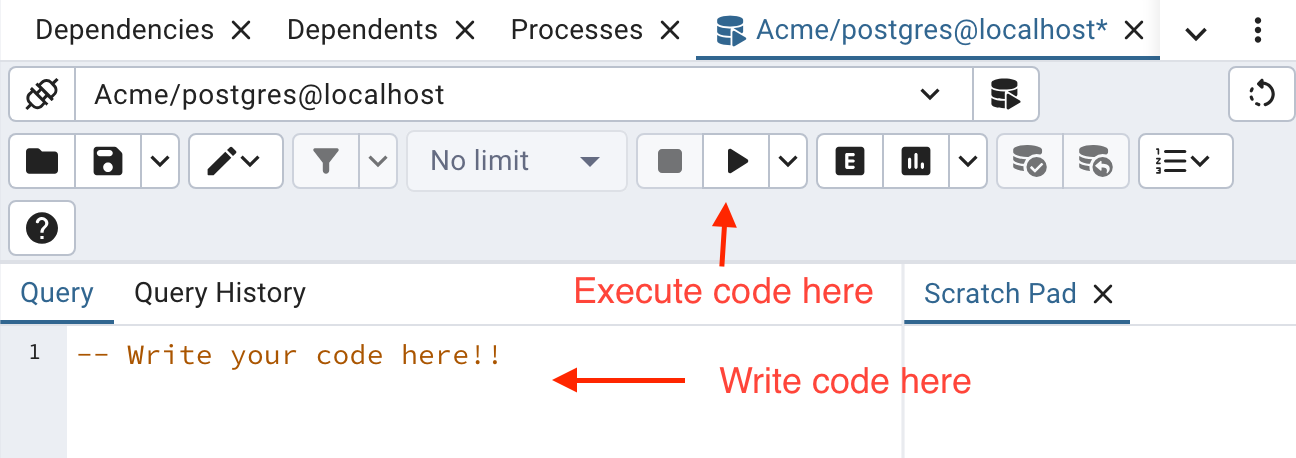
\includegraphics[width=0.7\textwidth]{content/1-relational-databases/figures/pgadmin/9.png}
    \caption{Write your code, and execute it}
    \label{fig:1.pgadmin9}
\end{figure}

Now that your machine is ready, and you have connected to the database, you are ready to start working with databases. The next chapter will guide you through the process of creating a database, and managing tables, as well as how to query the database.


% ******************************* Chapter: Relational Database Basics ****************************
\chapter{Relational Database Basics}
\label{chap:relational:relational-database-basics}
This chapter contains the basic building blocks to get started with basic relational databases.
It will explain the basic concepts of databases, and how to create, manage, and query a database.

\section{Creating your first database}
Creating a database is the first step in working with databases. This section will guide you through the process of creating a database. 

The following codesnippet shows the available syntax for the create database operation. The syntax is the same for all database management systems, but the options available might differ. The options available in PostgreSQL are shown in the example.

\begin{minted}[fontsize=\footnotesize]{postgresql}
    -- Creating a database with full syntax
    CREATE DATABASE database_name
    WITH
        [OWNER =  role_name]
        [TEMPLATE = template]
        [ENCODING = encoding]
        [LC_COLLATE = collate]
        [LC_CTYPE = ctype]
        [TABLESPACE = tablespace_name]
        [ALLOW_CONNECTIONS = true | false]
        [CONNECTION LIMIT = max_concurrent_connection]
        [IS_TEMPLATE = true | false ]
\end{minted}

The key element to understand here is that the name of the CREATE DATABASE statement and a database name of your choosing is mandatory, the WITH clause and everything after it is optional. If no parameters are set, the database will be created with default settings. Therefore, the simplest way to create a database is to run the following command:

\begin{minted}[fontsize=\footnotesize]{postgresql}
    -- Creating an ACME database with minimal syntax
    CREATE DATABASE Acme;
\end{minted}

Note that both examples you have seen until now, are also using comments. A double dash "--" creates a one-line comment, and a slash-star "/*" creates a multi-line comment. Comments are not executed, and are only there to help you understand the code. It does, however, make the code more readable and understandable, and is therefore a good practice to use comments.

If you wish to create a database with specific settings, you can use the WITH clause. The following example shows how to create a database with specific settings:

\begin{minted}[fontsize=\footnotesize]{postgresql}
    -- Creating a ACME database with enabled options
    CREATE DATABASE Acme 
    WITH
        OWNER = postgres
        CONNECTION LIMIT = 50;
        IS_TEMPLATE = false;
\end{minted}

\subsection{Altering and deleting databases}
If you wish an already existing database settings can be altered. The following example shows how to alter a database, and disable index scans (which is not recommended):

\begin{minted}[fontsize=\footnotesize]{postgresql}
    -- Alter Database Acme to disable index scans
    ALTER DATABASE Acme SET enable_indexscan TO off;
\end{minted}

The last missing component is how to delete a database. The following example shows how to delete a database. Beware that this is a permanent operation, and that all data in the database will be lost with no way to recover the data!

\begin{minted}[fontsize=\footnotesize]{postgresql}
    -- Delete a table
    DROP DATABASE Acme;
\end{minted}

\subsection{Switch databases}
It is also possible to switch between databases within the same script on most database management systems. Inside the script, one can freely change databases and run queries on different databases. The following example shows how to switch databases in in Microsoft SQL:

\begin{minted}[fontsize=\footnotesize]{sql}
    /* Change to database_name
     * This does not work with PostgreSQL */
    USE database_name;
\end{minted}

However, this does not work with PostgreSQL. PostgreSQL is implemented differently, and requires that you actively with your graphical user interface, or with the command line, switch to the database you want to work with. The following example shows how to switch databases in PostgreSQL from the command line using psql:

\begin{minted}[fontsize=\footnotesize]{psql}
    -- Change to database_name from psql command line
    \connect database_name
\end{minted}

\section{Datatypes in Databases}
When creating a table, you need to specify the data type for each column. Therefore, this section clarifies what datatypes are, and how they should be used, as well as some best practices. The data type specifies what type of data the column can hold. While databases support different datatypes, there are several common types that works between DBMS implementations. Table \ref{tab:1.postgresql-datatypes} shows the most commonly used data types in PostgreSQL.

\begin{table}[htb]
    \centering
    \resizebox{\textwidth}{!}{%
    \begin{tabular}{|l|l|}
    \hline
    \textbf{Data Type} & \textbf{Description} \\ \hline
    \textbf{BOOLEAN} & Logical Boolean (true/false) \\ \hline
    \textbf{CHAR(n)} & Fixed-length character string \\ \hline
    \textbf{VARCHAR(n)} & Variable-length character string \\ \hline
    \textbf{TEXT} & Variable-length character string \\ \hline
    \textbf{INTEGER} & Signed integer (4 bytes) \\ \hline
    \textbf{BIGINT} & Signed integer (8 bytes) \\ \hline
    \textbf{DECIMAL(precision, scale)} & Exact numeric of selectable precision \\ \hline
    \textbf{NUMERIC(precision, scale)} & Exact numeric of selectable precision \\ \hline
    \textbf{REAL} & Single precision floating-point number (4 bytes) \\ \hline
    \textbf{DOUBLE PRECISION} & Double precision floating-point number (8 bytes) \\ \hline
    \textbf{DATE} & Calendar date (year, month, day) \\ \hline
    \textbf{TIME} & Time of day (hour, minute, second) \\ \hline
    \textbf{TIMESTAMP} & Date and time (no time zone) \\ \hline
    \textbf{TIMESTAMPTZ} & Date and time (with time zone) \\ \hline
    \textbf{INTERVAL} & Time interval \\ \hline
    \textbf{UUID} & Universally unique identifier \\ \hline
    \textbf{XML} & XML data \\ \hline
    \textbf{JSON} & JSON data \\ \hline
    \textbf{ARRAY} & Array of any data type \\ \hline
    \end{tabular}%
    }
    \caption{Commonly used data types in PostgreSQL}
    \label{tab:1.postgresql-datatypes}
\end{table}

The datatypes are just some of the available types, and i recommend you read up on the documentation for the database management system you are using. The documentation will show you all the available datatypes, and how to use them.
You should get familiar with a few of the datatypes as they will be used the most often, and it is important you understand how they are used, and how they differ from each other. Examples of these datatypes are mainly within three areas: text, numbers, and dates.

Within the text area, you have the CHAR(n), VARCHAR(n), and TEXT datatypes. The CHAR(n) datatype is a fixed-length character string, and the VARCHAR(n) datatype is a variable-length character string. The TEXT datatype is a variable-length character string, and is used for large amounts of text. The difference between CHAR(n) and VARCHAR(n) is that CHAR(n) will always be n characters long, and will be padded with spaces if the text is shorter than n characters. VARCHAR(n) will only be as long as the text, and will not be padded with spaces. The TEXT datatype is used for large amounts of text, and is the most flexible of the three. However, my recommendation when learning databases is to use the VARCHAR(n) datatype, as it is flexible, and supports most scenarios. So for now, think of text as VARCHAR(n). Once you understand databases better, you will understand when to use the other datatypes.

The next datatype area to get familiar with is the numbers area. The INTEGER and BIGINT datatypes are used for whole numbers, and the DECIMAL(precision, scale) and NUMERIC(precision, scale) datatypes are used for decimal numbers. The difference between INTEGER and BIGINT is the size of the number they can hold. INTEGER can hold numbers from -2147483648 to 2147483647, and BIGINT can hold numbers from -9223372036854775808 to 9223372036854775807. The DECIMAL(precision, scale) and NUMERIC(precision, scale) datatypes are used for decimal numbers, and the difference between them is that DECIMAL is the same as NUMERIC, but the implementation can differ between database management systems. The precision is the total number of digits, and the scale is the number of digits to the right of the decimal point. So DECIMAL(5,2) can hold numbers from -999.99 to 999.99. My recommendation is to use INTEGER for whole numbers, and DECIMAL(precision, scale) for decimal numbers, and leave other options for for when those does not satisfy the requirements.

Lastly, the dates area is the last area to get familiar with. The DATE datatype is used for calendar dates (does not contain the concept of hours, minutes and seconds), and the TIME datatype is used for time of day (does not contain the concept of a date). The TIMESTAMP datatype is used for date and time, so it combines the two previous concepts, and the TIMESTAMPTZ datatype is used for date and time with time zone. The INTERVAL datatype is used to quantify the time between two dates or timestamps. My recommendation is to use the TIMESTAMP datatype for date and time, and the DATE datatype for calendar dates. The other datatypes are used for specific scenarios, and should be used when those scenarios are present.

\section{Constraints}
Another important concept to understand when working with databases is constraints. Without constraints it is impossible to make large scale consistent databases. Constraints are used to enforce rules on the data in the database. This section will guide you through the types of constraints that will be used in later sections. The available types of constrains are shown in \cref{tab:1.postgresql-constraints}. We are going to touch upon four of the above constraint types. Primary Keys, Foreign Keys, Unique, and Not Null. With Primary Keys, we are also going to touch upon the concept of composite keys.

\begin{table}[htb]
    \centering
    \resizebox{\textwidth}{!}{%
    \begin{tabular}{|l|l|}
    \hline
    \textbf{Constraint} & \textbf{Description} \\ \hline
    \textbf{NOT NULL} & Ensures that a column cannot have a NULL value \\ \hline
    \textbf{UNIQUE} & Ensures that all values in a column are different \\ \hline
    \textbf{PRIMARY KEY} & \makecell[l]{A combination of a NOT NULL and UNIQUE. \\Uniquely identifies each row in a table} \\ \hline
    \textbf{FOREIGN KEY} & Uniquely identifies a row/record in another table \\ \hline
    \textbf{CHECK} & Ensures that all values in a column satisfies a specific condition \\ \hline
    \textbf{EXCLUSION} & \makecell[l]{Ensures that if any two rows are compared on the \\ specified column or expression using the specified operator, \\at least one of the comparisons will return FALSE or NULL} \\ \hline
    \end{tabular}%
    }
    \caption{Commonly used constraints in PostgreSQL}
    \label{tab:1.postgresql-constraints}
\end{table}

\begin{itemize}
    \item \textbf{Primary Key:} A primary key is a field in a table which uniquely identifies each row/record in that table. It is a unique identifier for the rows in the table. A primary key cannot contain NULL values, and there can only be one primary key in a table. A primary key can be made up of one or more columns. When a primary key is made up of more than one column, it is called a composite key. Make sure your table \textbf{always} has a primary key, as it is the most important constraint in a table. With a primary key, you will often see a datatype of SERIAL, which is a special datatype that is used to auto increment the value of the column.
    \item \textbf{Foreign Key:} A foreign key is a field in a table that is a primary key in another table. It can be used to link two tables together. A foreign key can contain NULL values, unless otherwise specified, and there can be multiple foreign keys in a table. A foreign key is used to ensure that the value in the foreign key column exists in the primary key column in the other table. This is used to enforce referential integrity, and is used to link two tables together.
    \item \textbf{Unique:} A unique constraint is used to ensure that all values in a column are different. It is used to enforce the uniqueness of the values in a column, and is commonly used in conjunction with fields that contain an email address, or a username, to make sure that user does not exist multiple times, but of cause finds it use in other scenarios as well.
    \item \textbf{Not Null:} A not null constraint is used to ensure that a column cannot have a NULL value. What is a null value? A null value is a value that is not known, not available, or does not exist. It is different from a zero value or a field that contains spaces. A null value is used to represent a missing value, and is used to represent the absence of a value.
\end{itemize}

Now that you have a basic understanding of constraints, you are ready to start creating tables. The next section will guide you through the process of creating a table, and how to use the constraints you have learned about.

\section{Working with Tables}
Now that you have a basic understanding of databases, and how to create a database, datatypes and constraints that you will encounter in this section, you are ready to start creating tables. This section will guide you through the process of creating a table, and how to use the constraints you have learned about.

\subsection{Creating tables}
The following codesnippet shows the available syntax for the create table operation. The syntax is the same for all database management systems, but the options available might differ. The options available in PostgreSQL are shown in the example.

\begin{minted}[fontsize=\footnotesize]{postgresql}
    -- Create a table
    CREATE TABLE [IF NOT EXISTS] table_name (
        column1 datatype(length) column_constraint,
        column2 datatype(length) column_constraint,
        ...
        table_constraints
    );
\end{minted}

What is important to understand here is that the name of the CREATE TABLE statement and a table name of your choosing is mandatory, the IF NOT EXISTS clause is optional. Each line under the CREATE statement, defines a column in the table. The column name, the datatype, and the column constraint is mandatory, and the length is optional. The table constraints is also optional, and is used to define constraints on the table as a whole. Moving this example to a concrete implementation of a table, the example below shows how to create a table with the name account, and the columns user\_id, username, and password.

\begin{minted}[fontsize=\footnotesize]{postgresql}
    -- Create a table
    CREATE TABLE tableName (
        tableName_id SERIAL PRIMARY KEY, -- auto incrementing id
        username VARCHAR (50) UNIQUE NOT NULL, -- unique username
        password VARCHAR (250) NOT NULL -- never store in plain text
    );
\end{minted}

Specifically, from the CREATE statement, here we define a table name. The next line defines a PRIMARY KEY to ensure the line itself is unique and can be refered to. This line employs the SERIAL datatype to auto increment the value of the column with each new row that is added to the table. The line below defines a username that can be the maximum length of 50 characters, but defines that it must be defined using NOT NULL, and that no other row in the table can have the same value. The last line defines a password that can be the maximum length of 250 characters, but defines it must be set as the NOT NULL constraint is set. This is an example, never store passwords in plain text, and always use a hashing algorithm to hash the password before storing it in the database.

The next example shows how to create a table with a foreign key. The example shows how to create a table with the name blog\_entries, and the columns id, header, body, and created\_by. The created\_by column is a foreign key that references the id column in the account table. 

\begin{minted}[fontsize=\footnotesize]{postgresql}
    -- Create account table
    CREATE TABLE account (
        id serial PRIMARY KEY,
        username VARCHAR (50) UNIQUE NOT NULL,
        created_on TIMESTAMP NOT NULL, 
        last_login TIMESTAMP
    );
    
    /* Create blog entries table
     * the created_by column references the 
     * id column in the account table */
    CREATE TABLE blog_entries (
        id serial PRIMARY KEY, 
        header VARCHAR (255) NOT NULL,
        body TEXT NOT NULL,
        created_by INTEGER NOT NULL REFERENCES account (id)
    );
\end{minted}

Note how a foreign key is defined, and how it REFERENCES the id column in the account table, and does not use its definition as a keyword. So, REFERENCES table(id), is the actual implementation of a FOREIGN KEY. This ensures a blog post cannot be created without a user to be associated with it. This also means that if a user is deleted and cascading deletions are enabled, all blog posts associated with that user will also be deleted. Normally tough, this is not the case, and a deletion will fail until all blog entries from that account is deleted.

Now that we are able to create tables, the question arises, what happens if something was done wrong, and the table needs to be altered or deleted? 

\subsection{Altering tables}
If you wish to alter a table, you can use the ALTER TABLE statement. The following codesnippet shows the available syntax for the alter table operation. The syntax is the same for all database management systems, but the options available might differ. The options available in PostgreSQL are shown in the example.

\begin{minted}[fontsize=\footnotesize]{postgresql}
    -- Alter a table
    ALTER TABLE table_name action;
\end{minted}

As you can see at this point, the alter command does not specify what action to take. The action is specified in the next line, and the available actions are shown in \cref{tab:1.postgresql-alter-table-actions}.

\begin{table}[htb]
    \centering
    \resizebox{\textwidth}{!}{%
    \begin{tabular}{|l|l|}
    \hline
    \textbf{Action} & \textbf{Description} \\ \hline
    \textbf{ADD} & Adds a new column to the table \\ \hline
    \textbf{DROP} & Removes a column from the table \\ \hline
    \textbf{ALTER} & Modifies the data type of a column in the table \\ \hline
    \textbf{RENAME} & Renames a column in the table \\ \hline
    \textbf{RENAME TO} & Renames the table \\ \hline
    \textbf{SET} & Changes the value of a column in the table \\ \hline
    \textbf{RESET} & Resets the value of a column in the table \\ \hline
    \textbf{OWNER TO} & Changes the owner of the table \\ \hline
    \end{tabular}%
    }
    \caption{Available actions for the ALTER TABLE statement}
    \label{tab:1.postgresql-alter-table-actions}
\end{table}

From this point on, the task comes to find the correct action to take, and the correct syntax to use. The following example shows how to add a column to a table.

\begin{minted}[fontsize=\footnotesize]{postgresql}
    -- Add a column to a table
    ALTER TABLE table_name 
    ADD COLUMN column_name datatype column_constraint;
\end{minted}

For specific examples of how to use ALTER for each action, i recommend visting \url{https://www.postgresqltutorial.com/postgresql-tutorial/postgresql-alter-table/} and read up on the documentation for the database management system you are using. The documentation will show you all the available actions, and how to use them.


\subsection{Deleting tables}
Compared to altering tables, deleting tables is a more straightforward operation. The following codesnippet shows the available syntax for the delete table operation. The syntax is the same for all database management systems, but the options available might differ. The options available in PostgreSQL are shown in the example.

\begin{minted}[fontsize=\footnotesize]{postgresql}
    -- Delete a table
    DROP TABLE [IF EXISTS] table_name 
    [CASCADE | RESTRICT];
\end{minted}

Here the name of the DROP TABLE statement and a table name of your choosing is mandatory, the IF EXISTS clause is optional, and the CASCADE | RESTRICT clause is also optional. The CASCADE | RESTRICT clause is used to specify what to do if the table has dependencies. If the table has dependencies, and CASCADE is specified, the table and all its dependencies will be deleted. If the table has dependencies, and RESTRICT is specified, the table will not be deleted. The following example shows how to delete a table and all of its dependencies.

\begin{minted}[fontsize=\footnotesize]{postgresql}
    -- Delete a table and all of its dependencies
    DROP TABLE table_name CASCADE;
\end{minted}

At this point, you can now create databases, tables, and alter and delete tables. You are now ready to start working with databases. The next section will guide you through the process of inserting data into a table, and how to query the data from the table.

\section{CRUD Operations}

\section{Joins and querying related tables}

% ******************************* Chapter: ER, EER Modeling and Database Design ****************************
\chapter{ER, EER Modeling and Database Design}
\label{chap:relational:eer-modeling-and-database-design}
This chapter teaches basic ER and ER modelling, and how to design a database from an ER model.

\section{The purpose of ER and EER modeling}
\section{Diagram Elements}
\section{ER versus EER modeling}
\section{Mapping to tables}

% ******************************* Chapter: Database Normalization ****************************
\chapter{Database Normalization}
\label{chap:relational:database-normalization}
This chapter teaches database normalization to the 4th normal form.

\section{What is database normalization?}
\section{Shorthand techniques}
\section{First normal form}
\section{Second normal form}
\section{Third normal form}
\section{Fourth normal form}
\section{Normalization of other formats}

% ******************************* Chapter: Advanced Relational Databases ****************************
\chapter{Advanced Relational Databases}
\label{chap:relational:advanced-relational-databases}
This chapter teaches advanced relational database concepts.

\section{Transactions}
\section{Indexes}
\section{Views}
\section{Stored Procedures}
\section{Triggers}
\section{User Defined Functions}
\section{Security}
\section{Performance Tuning}


